\chapter{\IfLanguageName{dutch}{Resultaten}{Results}}%
\label{ch:resultaten}

In dit hoofdstuk worden de resultaten uit de requirementsanalyse, vergelijkende studie en de ontwikkeling van het prototype besproken. 

Dit hoofdstuk van het onderzoek bespreekt de resultaten van de drie onderzoeksmethoden. Allereerst geeft het onderzoek de resultaten van de requirementsanalyse, door middel van een bespreking van het toegepaste moscow-schema op de geteste tools. Daarna staat het onderzoek stil bij de objectieve en subjectieve leesgraadscores afgeleid uit de vergelijkende studie. Tot slot bespreekt het onderzoek het ontwikkelde prototype, alsook hoe dit prototype staat tegenover andere tools. De aftoetsing gebeurt op basis van de functionaliteiten voor gepersonaliseerde ATS op maat voor scholieren met dyslexie bij het begrijpend lezen van wetenschappelijke artikelen. 

\section{Ontbrekende functies bij AI-toepassingen}

Op basis van de testen kan de volgende criteria worden afgetoetst, weergegeven in tabel \ref{table:afgetoetste-criteria}. Alle labels voor de \textit{must-haves} staan vetgedrukt.


\medspace

Alle geteste toepassingen, buiten O4 en O5, laten gebruikers toe om wetenschappelijk artikelen als pdf opladen. Figuur \ref{img:scispace-example} toont hoe O2 gebruikers in het oorspronkelijke bestand kan laten werken. O4 en O5 beschikken enkel over een \textit{plain-text} invoermethode. O2 en O5 kunnen online wetenschappelijke artikelen via URL, maar dit gebeurt echter bij één van de twee uitgeteste wetenschappelijke artikelen.

\begin{figure}[H]
	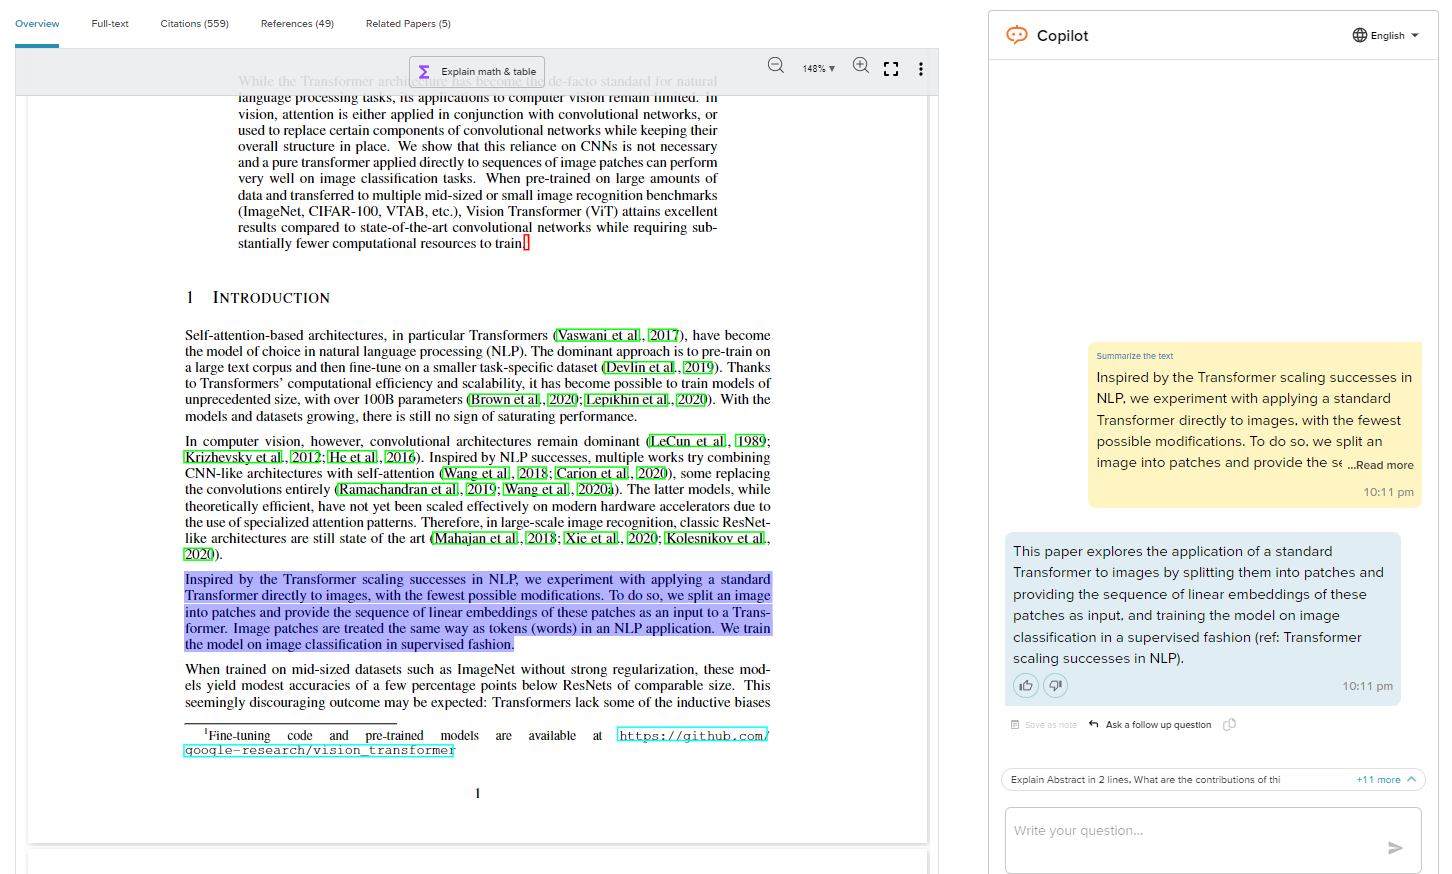
\includegraphics{img/typeset-example.png}
	\caption{Informatie opvragen van een wetenschappelijk artikel met SciSpace}
	\label{img:scispace-example}
\end{figure}

% Lexicale vereenvoudiging
Alle uitgeteste tools passen moeilijke woorden aan naar een eenvoudiger alternatief. O1, O3, O4 en O5 kunnen een extra definitie aan de woorden toevoegen, maar enkel wanneer er geen eenvoudiger alternatief is. Figuur \ref{img:simplish-output} toont hoe O1 een extra definitie in de voetnoot plaatst. Figuur \ref{img:scholarcy} toont aan dat O3 op taalniveau de doelgroep probeert in te schatten met \textit{rewordifying level}. O4 en O5 passen de doelgroep aan naargelang de meegegeven doelgroep in de prompt. Andere uitgeteste tools passen de woorden aan, maar bieden geen transparantie over de inschatting van de doelgroep.

\begin{figure}[H]
	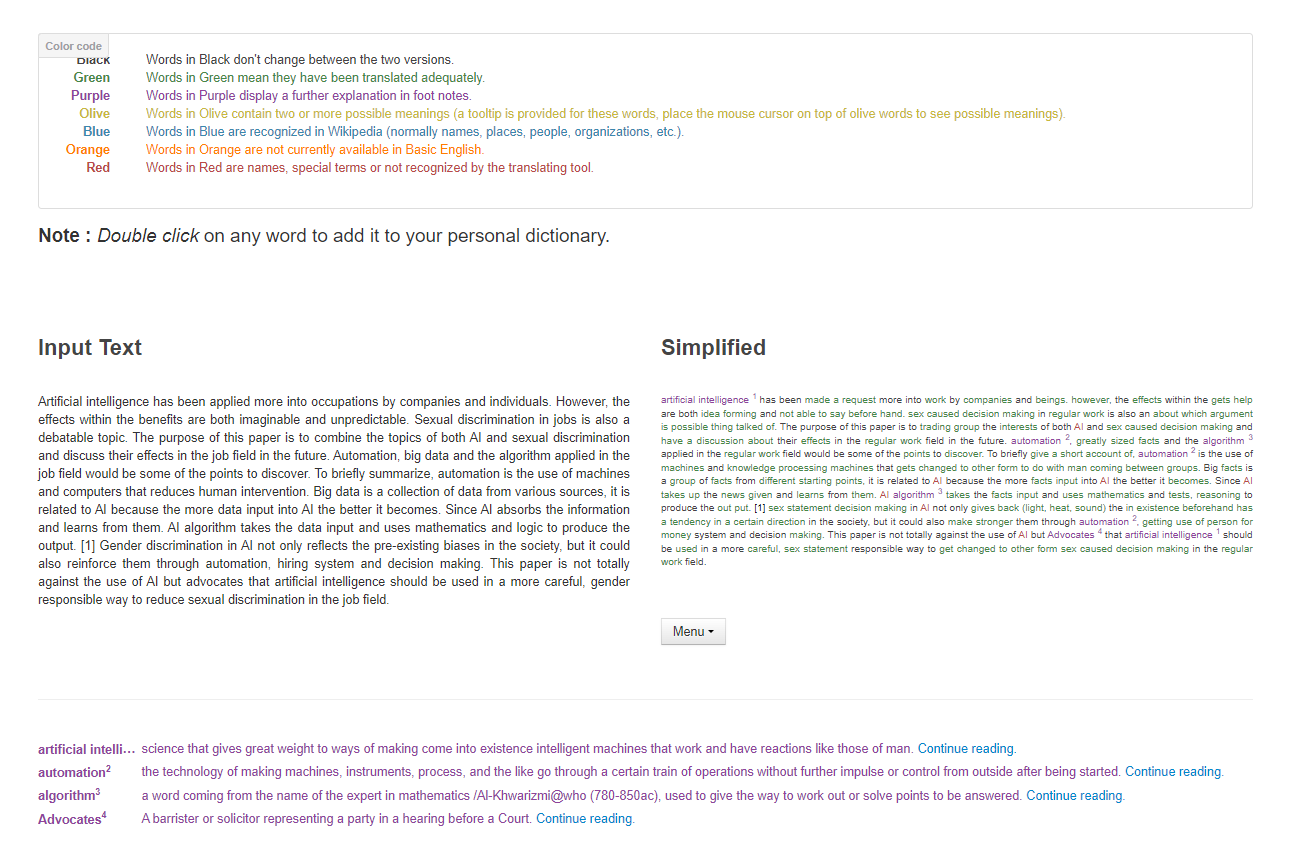
\includegraphics[width=\linewidth]{img/simplish-output.png}
	\caption{Illustratie van de tekstanalyse bij Simplish na een tekstvereenvoudiging.}
	\label{img:simplish-output}
\end{figure}
	
\begin{figure}[H]
		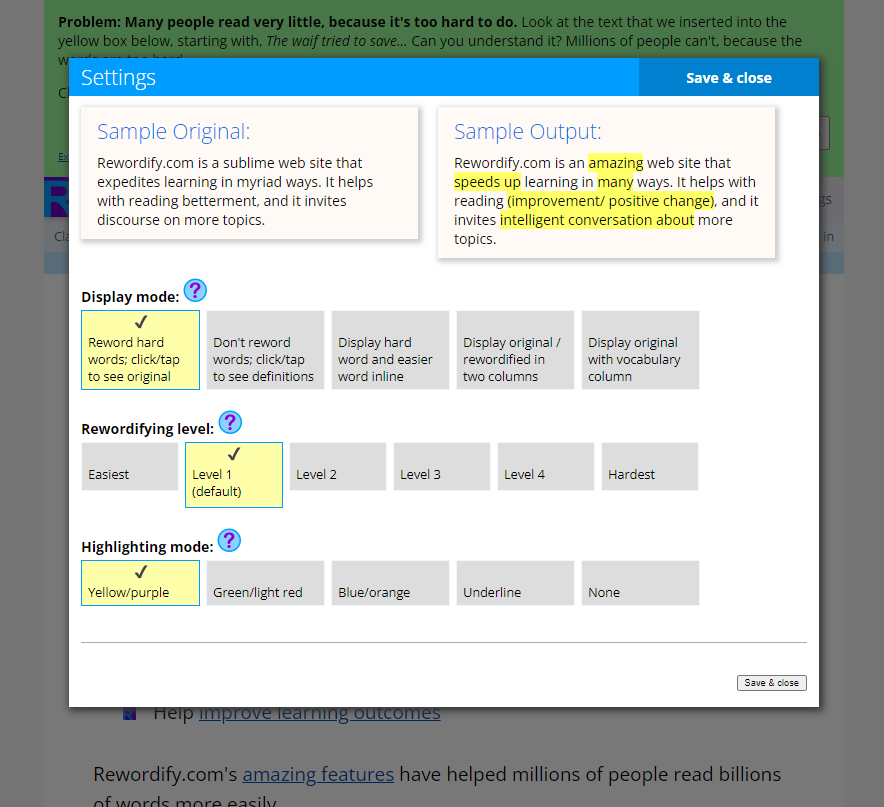
\includegraphics[width=\linewidth]{img/scholarcy-attempt.png}
		\caption{Illustratie van de tekstanalyse bij Rewordify.}
		\label{img:scholarcy}
\end{figure}

\medspace

% Woordenlijst

E1, E2, E3 en O1 kunnen woorden- en synoniemenlijsten genereren. De gebruiker moet hier de moeilijke woorden handmatig selecteren. Nadien bouwt de toepassing een woordenlijst. E1 geeft de eindgebruiker de keuze waarvan E1 de definitie moet halen. O1 geeft het type woord, zoals adjectieven of werkwoord, ook mee in de woordenlijst. O4 en O5 kunnen enkel een woordenlijst genereren na een expliciete prompt. Zowel handmatige als automatische woordselectie resulteren met de geteste prompt in een woordenlijst. Andere tools zijn niet in staat om een woordenlijst te genereren. De inschatting van de doelgroep bij deze moeilijke woorden gebeurt enkel manueel.

\medspace

E1, E2 en E3 reiken de \textit{must-have} opmaakopties aan binnen de toepassing. Andere tools ontbreken personaliseerbare opmaakopties en bieden een statische webweergave aan. E1, E2 en E3 bieden manieren aan om de aangepaste documenten op te slaan als PDF. Ten slotte biedt geen uitgeteste tool personaliseerbare opmaakopties voor de uitvoerbestanden aan. 

\medspace

E1, E2 en E3 kunnen geen SS-technieken toepassen op de oorspronkelijke tekst. Overige uitgeteste tools kunnen zinnen inkorten door ze te splitsen. Geen van de uitgeteste tools is in staat om automatisch de tekst naar de actieve vorm te schrijven. O4 en O5 kunnen zinnen omvormen naar de actieve stem, maar enkel als de tool een extra voornaamwoord of onderwerp in de prompt meekrijgt. O4 en O5 kunnen onregelmatige werkwoorden wegwerken. E1, E2 en E3 kunnen een extraherende samenvatting van de tekst maken, maar enkel na een handmatige selectie van de zinnen. 

\medspace

Tot slot slaagt enkel O4 en O5 erin om de tekst te herschrijven als opsomming of tabel. De andere uitgeteste tools kunnen dit niet automatisch doen.


\begin{table}[H]
	\centering
	\begin{tabular}{ | m{8cm} | m{0.5cm} | m{0.5cm} | m{0.5cm} | m{0.5cm} | m{0.5cm} | m{0.5cm} | m{1cm} | m{1cm} | }
		\hline
		\textbf{Richtlijn} & \textbf{E1} & \textbf{E2} & \textbf{E3} & \textbf{O1} & \textbf{O2} & \textbf{O3} & \textbf{O4} & \textbf{O5} \\ \hline
		Rekening houden met doelgroep & - & - & - & - & - & - & P2 & P2 \\ \hline
		Woorden met minder lettergrepen gebruiken & - & X & - & X & - & - & P1-6 & P1-6 \\ \hline
		Extra uitleg schrijven bij zinnen & - & X & - & - & - & - & P1-3 & P1-3 \\ \hline
		Paragrafen herschrijven zodat ze eerst uitleg geven op een high-level niveau & - & - & - & - & - & - & P2 & P2 \\ \hline
		Woordenlijst aanmaken & X & X & X & X & - & - & P6 & P6 \\ \hline
		Synoniemenlijst aanmaken & - & X & - & - & - & - & P6 & P6 \\ \hline
		Idiomen vervangen door eenvoudigere synoniemen & - & - & - & X & - & - & P1-3,6 & P1-3,6 \\ \hline
		Zinnen inkorten & - & - & - & X & X & X & P3-5 & P3-5 \\ \hline
		Verwijswoorden aanpassen & - & - & - & - & - & - & P3 & P3 \\ \hline
		Voorzetseluitdrukkingen aanpassen & - & - & - & - & - & - & P3 & P3 \\ \hline
		Samengestelde werkwoorden aanpassen & - & - & - & - & - & - & P3 & P3 \\ \hline
		Actieve stem toepassen & - & - & - & - & - & - & - & - \\ \hline
		Enkel regelmatige werkwoorden gebruiken & - & - & - & - & - & - & P3 & P3 \\ \hline
		Achtergrondkleur aanpassen & X & X & X & - & - & - & - & - \\ \hline
		Woord- en karakterspatiëring & - & X & X & - & - & - & - & - \\ \hline
		Consistente lay-out & X & X & X & - & - & - & P1-6 & P1-6 \\ \hline
		Duidelijk zichtbare koppenstructuur & - & - & - & - & - & - & - & - \\ \hline
		Huidige positie benadrukken & - & - & - & - & - & - & - & - \\ \hline
		Waarschuwingen geven omtrent formulieren en sessies & - & - & - & X & - & X & - & - \\ \hline
		Inhoud visueel groeperen & - & X & X & - & - & - & - & - \\ \hline
		Tekst herschrijven als tabel & - & - & - & - & - & - & P4, P6 & P4, P6 \\ \hline
		Tekst herschrijven als opsomming & - & - & - & - & - & - & P5 & P5 \\ \hline
		Artikel opladen als PDF & X & X & X & X & X & X & - & - \\ \hline
		Artikel opladen als \textit{plain-text} & - & - & - & - & - & - & P1-6 & P1-6 \\ \hline
		Artikel opladen via link & - & - & - & - & X* & - & P1-6* & - \\ \hline
	\end{tabular}
	\caption{Afgetoetste criteria volgens de experimenten.}
	\label{table:afgetoetste-criteria}
\end{table}


\section{Geschikte taalmodel voor gepersonaliseerde tekstvereenvoudiging met ATS}

De vergelijkende studie evalueert de uitvoer van de uitgeteste taallmodellen, opgesomd in \ref{table:vergelijkende-studie-taalmodellen}, met een subjectieve en een objectieve benadering. Zo achterhaalt deze onderzoeksmethode welk taalmodel of LLM beter aansluit bij het aanbieden van gepersonaliseerde ATS voor scholieren met dyslexie in de derde graad van het middelbaar onderwijs. 

\medspace

Tabel \ref{table:resultaten-aantal-zinnen} geeft het aantal zinnen per (vereenvoudigd) artikel. De MTS-referentieteksten bevatten minder zinnen dan het oorspronkelijk artikel. Het aantal zinnen na ATS met T1, T2 en T3 is gehalveerd tot minder dan een kwart van oorspronkelijke hoeveelheid zinnen. Enkel T4P2 genereert meer zinnen dan de oorspronkelijke versie van A1 na ATS. T4P2 genereert bij zowel A1 als A2 meer zinnen vergeleken met de andere geteste taalmodellen. T2 daarentegen genereert bij beide artikelen het minst aantal zinnen.

\medspace

Figuren \ref{img:boxplot-min-max-avg-words-a1} en \ref{img:boxplot-min-max-avg-words-a2} tonen de verdeling tussen het aantal gebruikte woorden per zin per taalmodel. Zo scoren alle artikelen gem

Daarnaast gebruiken T1, T2 en T3 gemiddeld minder woorden per zin dan het oorspronkelijke artikel. Alleen P3 van T4 slaagt erin om gemiddeld minder woorden per zin te gebruiken dan de oorspronkelijke en de referentieteksten van zowel leerlingen en de referentieteksten van leerkrachten, vergeleken met P1 en P2 die elk gemiddeld meer dan 19 woorden per zin gebruiken, zoals te zien is in figuren . 

\begin{table}[h]
	\centering
	\begin{tabular}{ | m{3cm} | m{3cm} | m{3cm} | } 
		\hline
		\textbf{Bron} & \textbf{#Zinnen in A1} & \textbf{#Zinnen in A2} \\
		\hline
		Oorspronkelijk & 78  & 159 \\ 
		\hline
		MTS (door leerkracht) & 43 & 45 \\
		\hline
		MTS (door leerling) & n.v.t. & 50 \\
		\hline
		T1 & 26 & 24 \\
		\hline
		T2 & 11 & 7 \\
		\hline
		T3 & 67 & 130 \\
		\hline
		T4 P1 & 61 & 98 \\
		\hline
		T4 P2 & 89 & 133 \\
		\hline
		T4 P3 & 39 & 55 \\
		\hline
	\end{tabular}
	\label{table:resultaten-aantal-zinnen}
	\caption{Aantal zinnen (gemeten met Spacy sentence embeddings) per tekst.}
\end{table}

\begin{figure}
	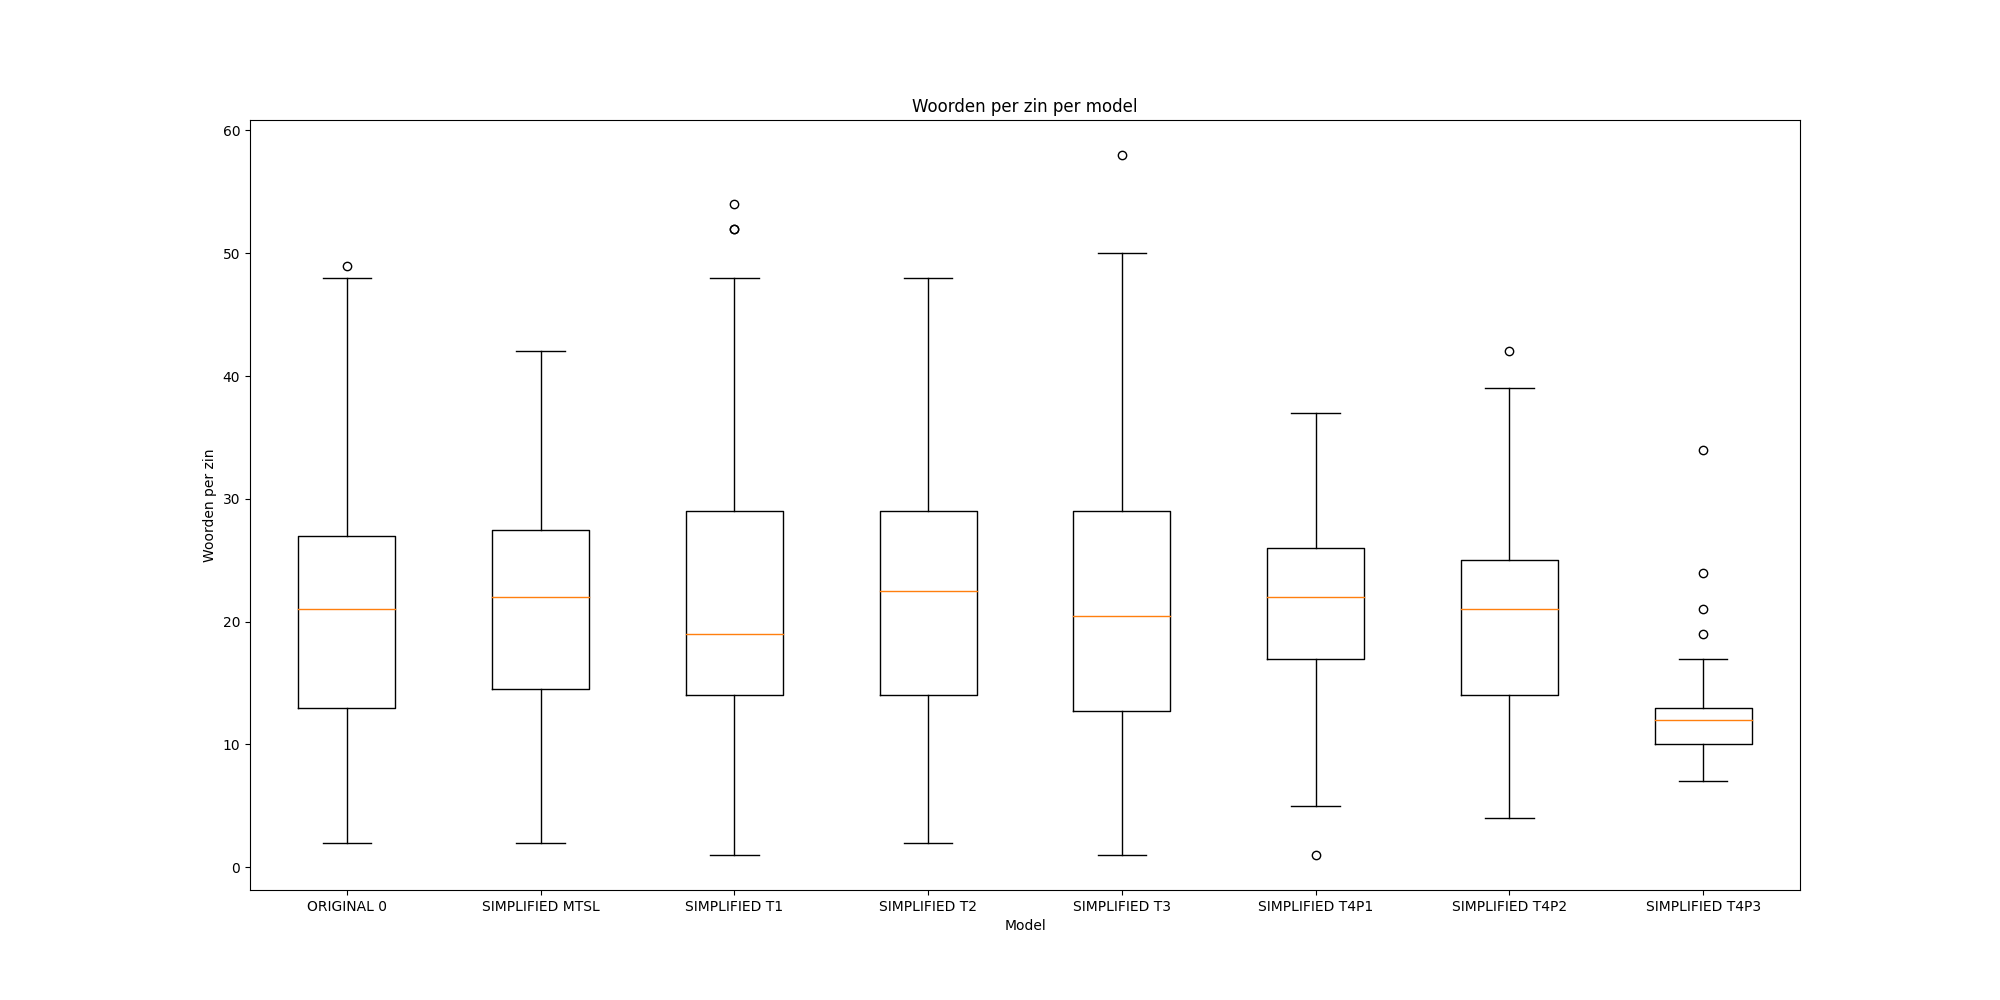
\includegraphics[width=\linewidth]{img/boxplot-avg-a1.png}
	\caption{Overzicht van het minimum, maximum en gemiddeld aantal woorden per zin per model in A1.}
	\label{img:boxplot-min-max-avg-words-a1}
\end{figure}

\begin{figure}
	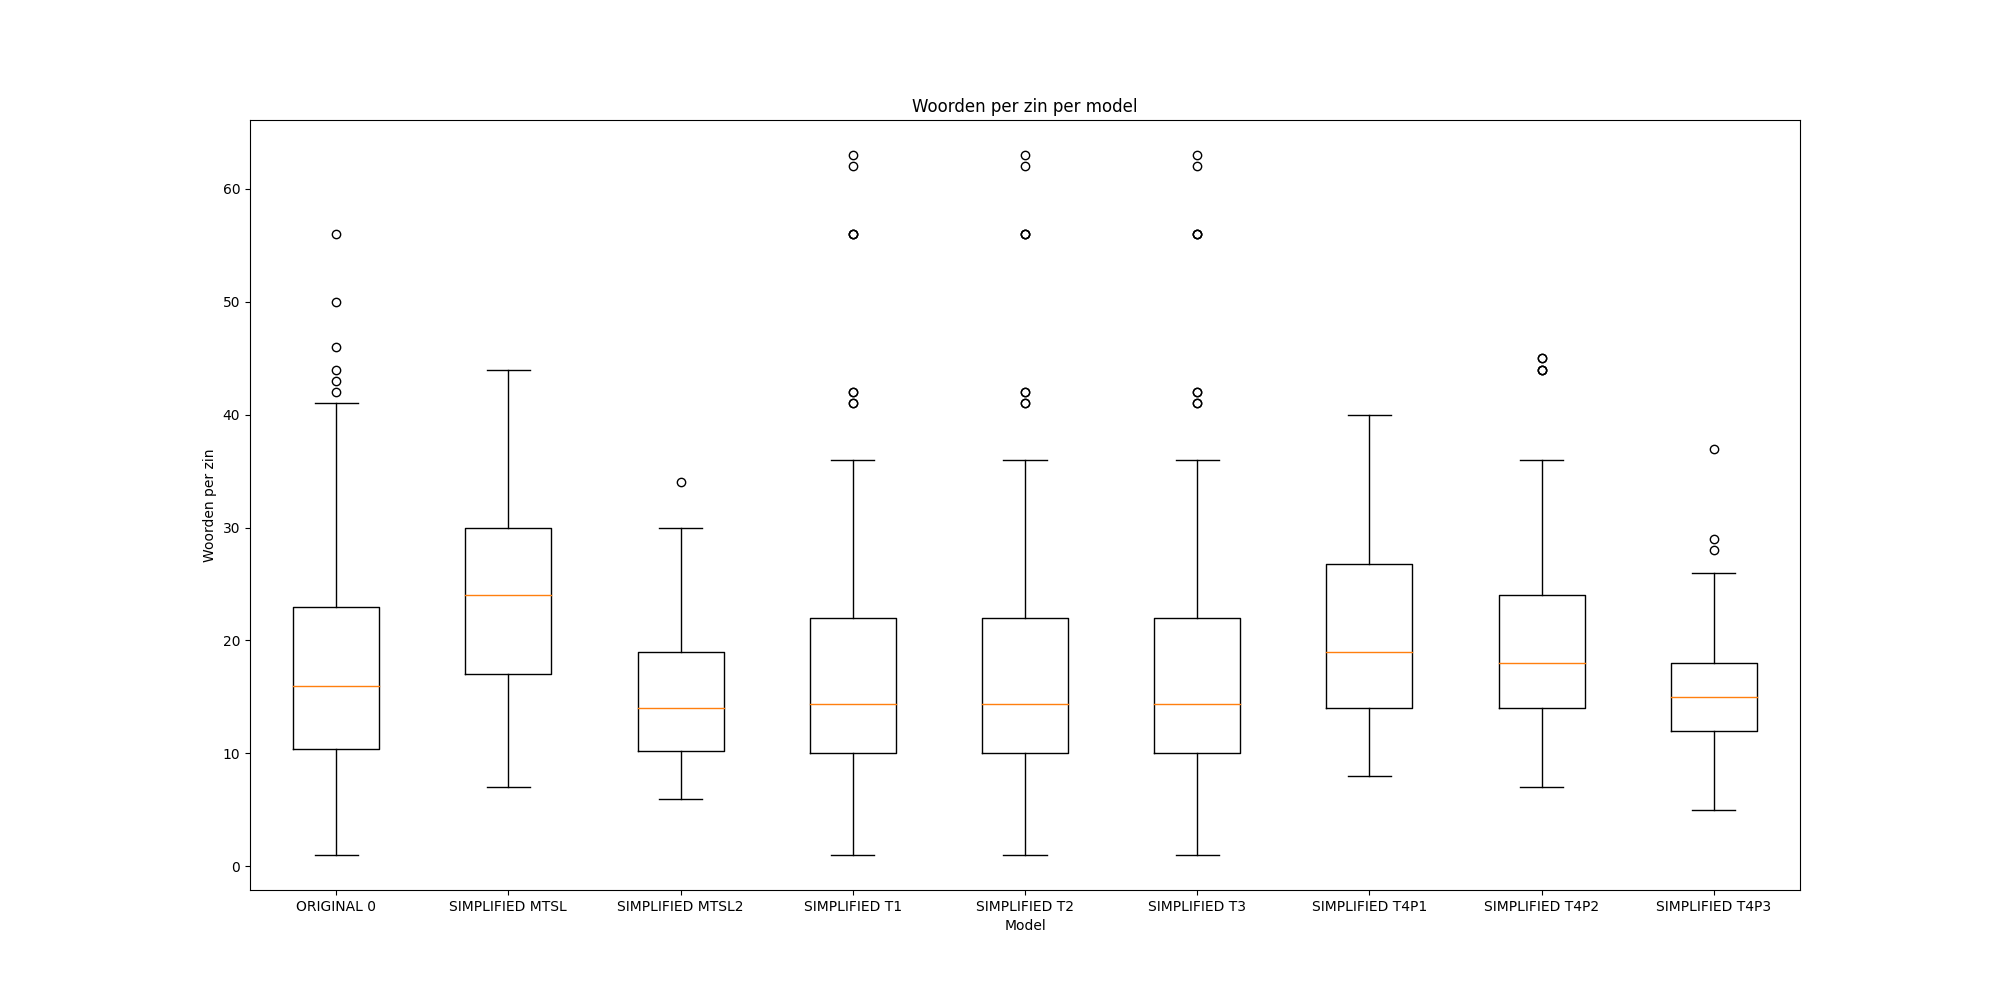
\includegraphics[width=\linewidth]{img/boxplot-avg-a2.png}
	\caption{Overzicht van het minimum, maximum en gemiddeld aantal woorden per zin per model in A2.}
	\label{img:boxplot-min-max-avg-words-a2}
\end{figure}

De FRE-scores van alle geteste taalmodellen en MTS-referentieteksten zijn niet significant hoger of lager dan die van het oorspronkelijke wetenschappelijke artikel, zoals weergegeven in figuren \ref{img:boxplot-fre-a1} en \ref{img:boxplot-fre-a2}. Daarnaast zijn de FOG-scores niet significant hoger of lager bij de vereenvoudigde wetenschappelijke artikelen, zoals aangegeven in figuren \ref{img:boxplot-fog-a1} en \ref{img:boxplot-fog-a2}. 


\begin{figure}
	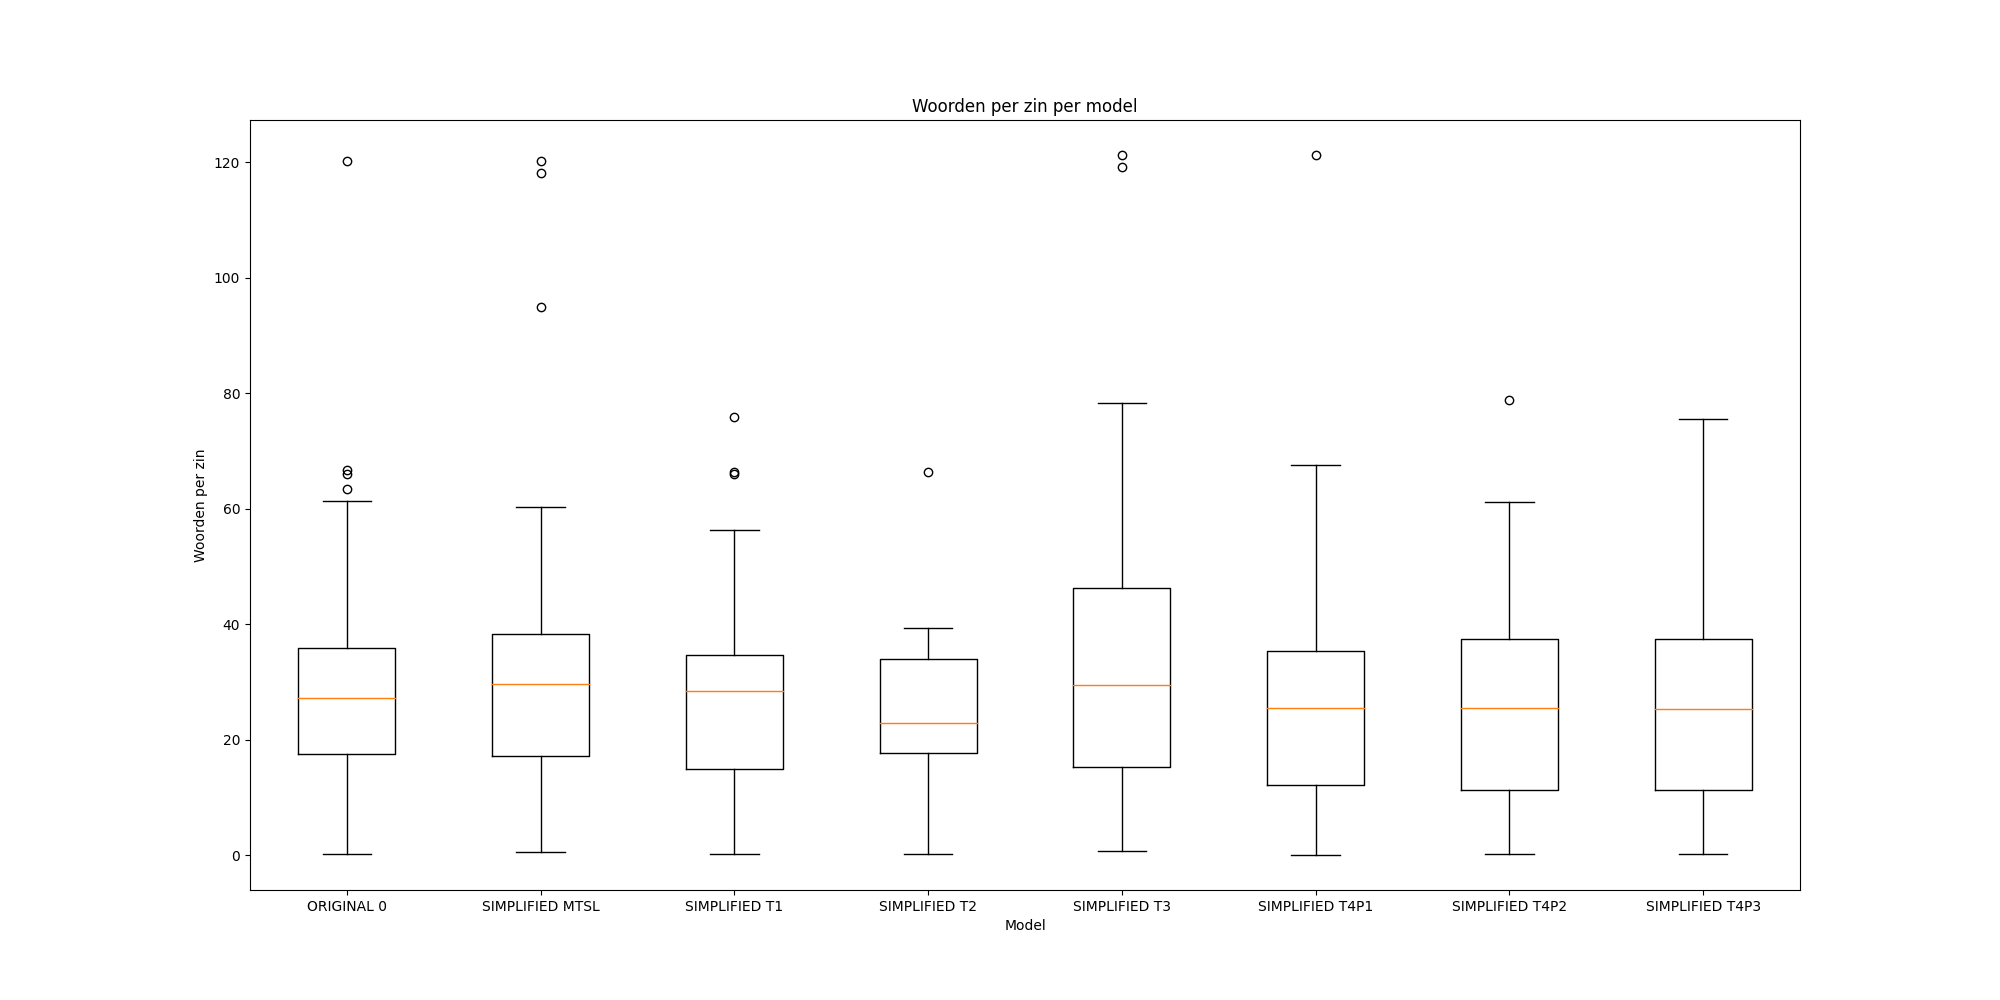
\includegraphics[width=\linewidth]{img/boxplot-fre-a1.png}
	\caption{Boxplot van de FRE-scores voor A1.}
	\label{img:boxplot-fre-a1}
\end{figure}

\begin{figure}
	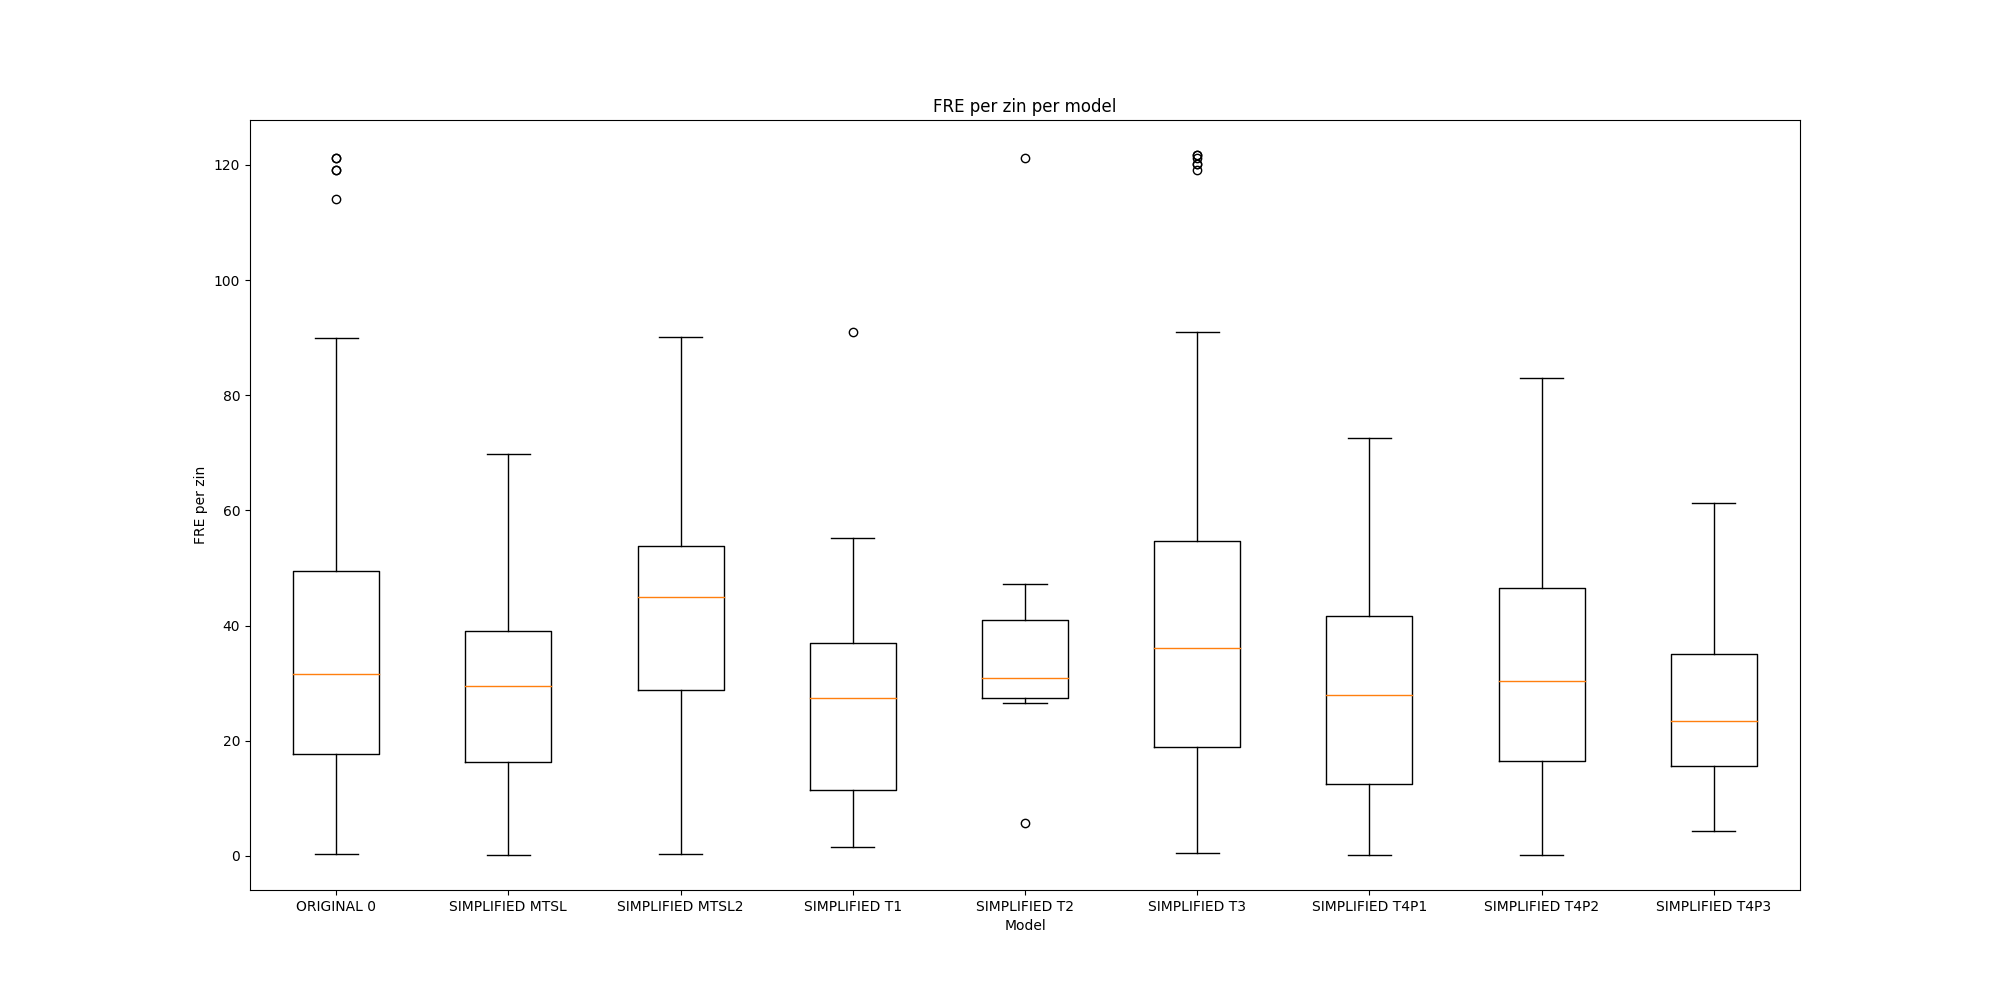
\includegraphics[width=\linewidth]{img/boxplot-fre-a2.png}
	\caption{Boxplot van de FRE-scores voor A2.}
	\label{img:boxplot-fre-a2}
\end{figure}

\begin{figure}
	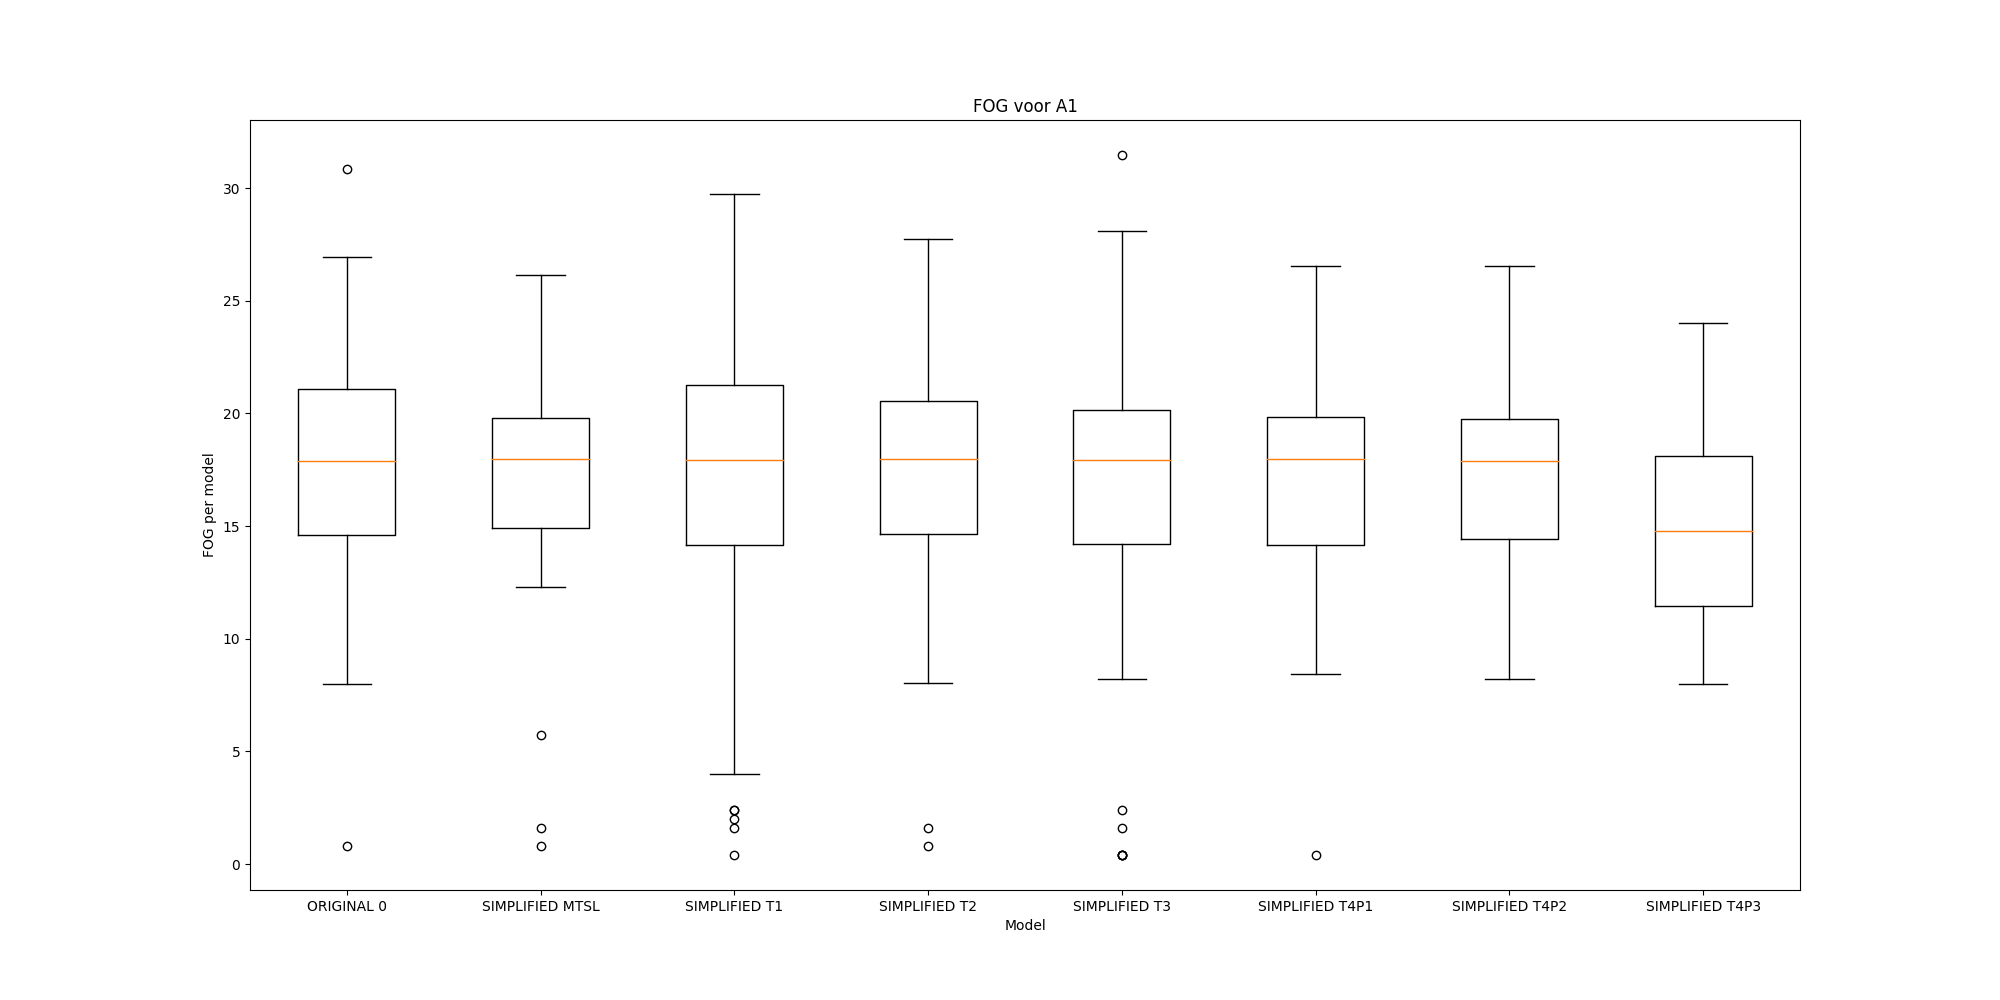
\includegraphics[width=\linewidth]{img/boxplot-fog-a1.png}
	\caption{Boxplot van de FOG-scores voor A1.}
	\label{img:boxplot-fog-a1}
\end{figure}

\begin{figure}
	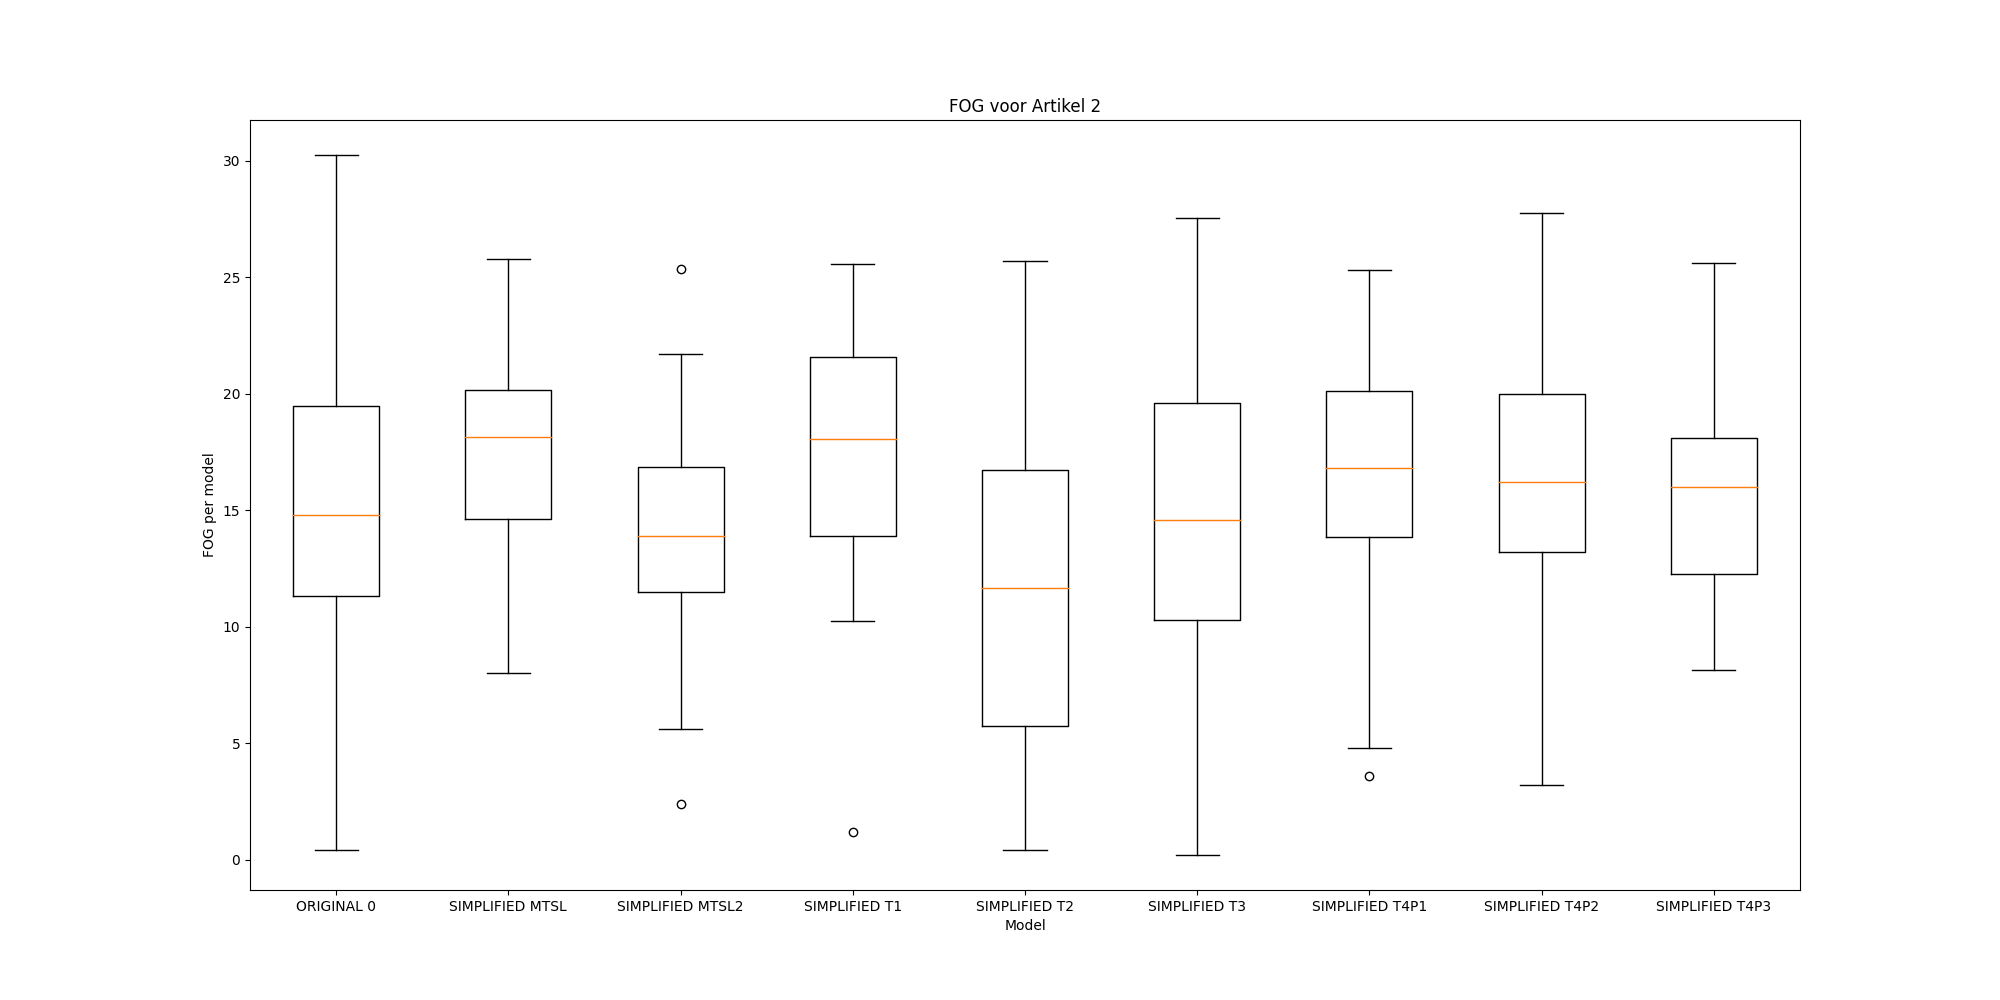
\includegraphics[width=\linewidth]{img/boxplot-fog-a2.png}
	\caption{Boxplot van de FOG-scores voor A2.}
	\label{img:boxplot-fog-a2}
\end{figure}

T1, T2 en T3 gebruiken bij zowel A1 als A2 langere woorden vergeleken met de oorspronkelijke tekst, in tegenstelling tot alle T4 prompts die wel langere woorden wegwerken en zo een gelijk resultaat bekomen als de MTS referentieteksten. Deze verhouding wordt aangewezen in figuren \ref{img:violinplot-long-a1} en \ref{img:violinplot-long-a2}. Daarnaast vervangen T1, T2 en T3 ook minder complexe woorden vergeleken met T4 en de MTS-referentietekst. Dit verschil wordt geïllustreerd in figuren \ref{img:violinplot-complex-a1} en \ref{img:violinplot-complex-a2}.

\begin{figure}
	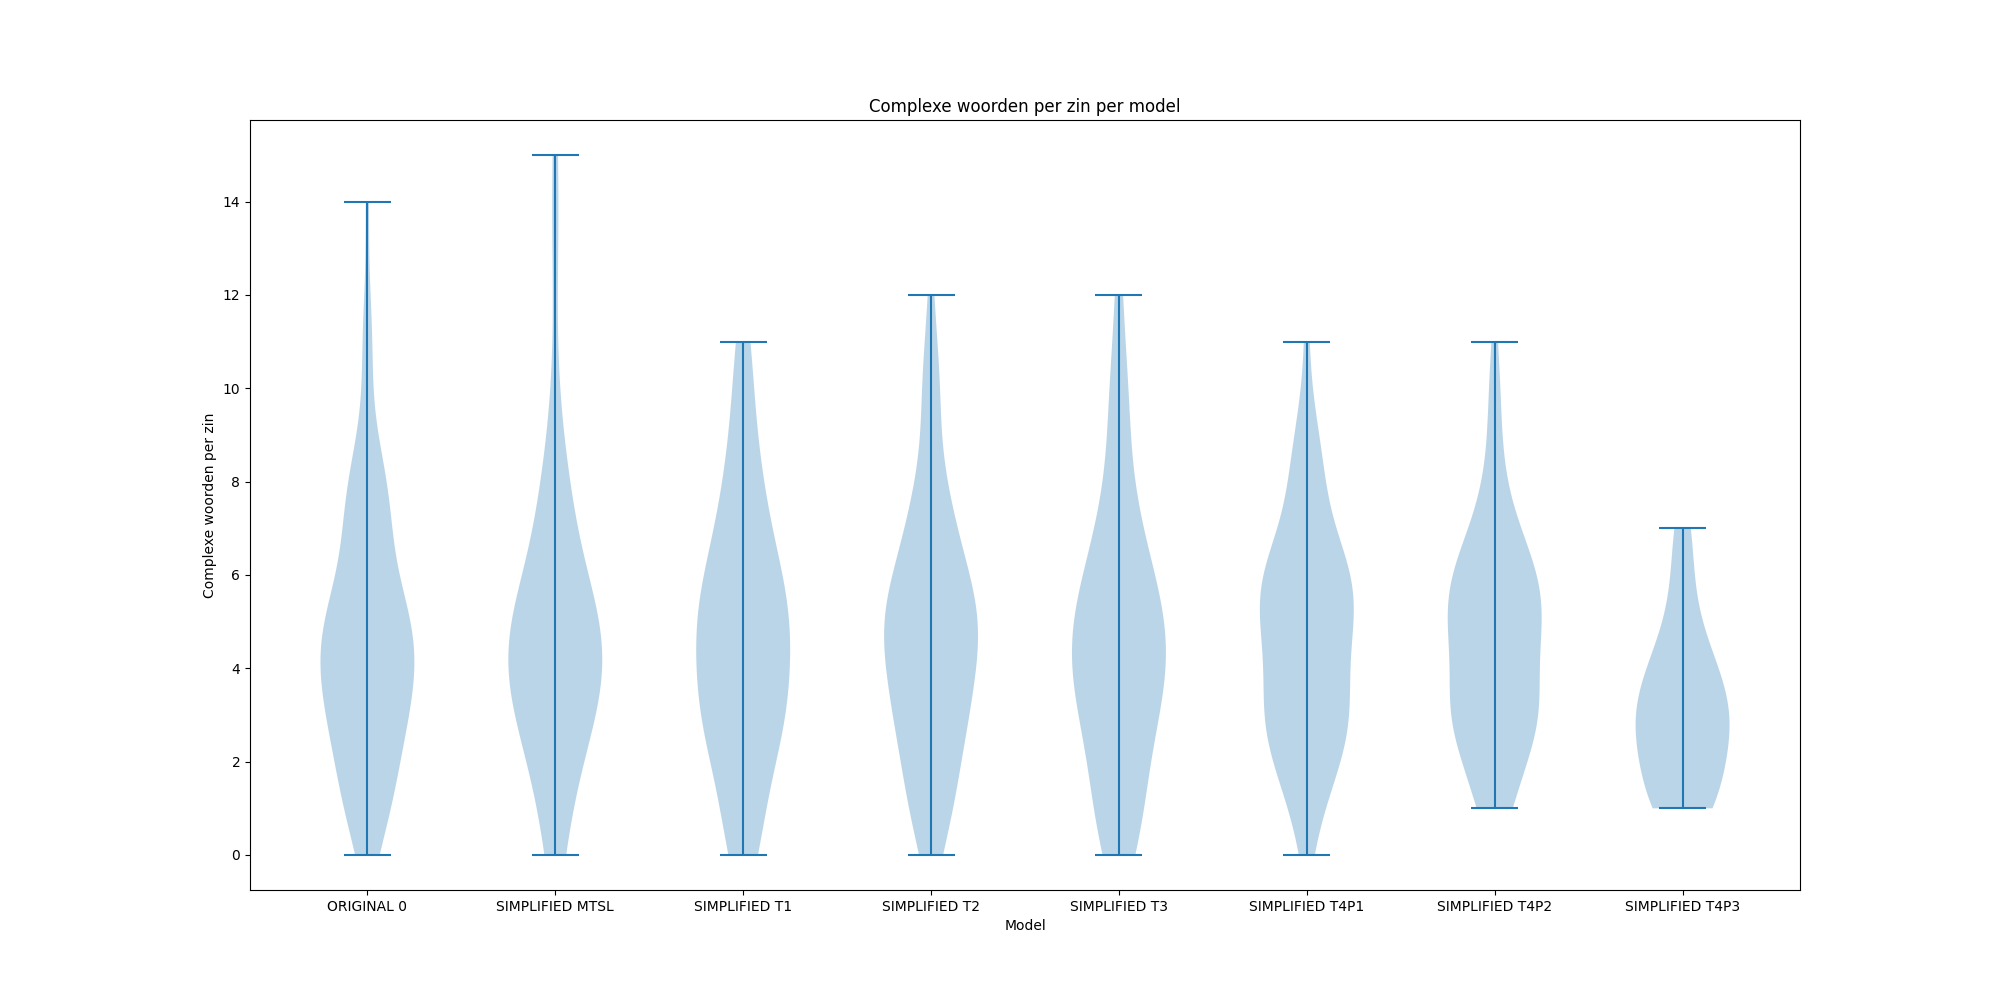
\includegraphics[width=\linewidth]{img/violinplot-complex-a1.png}
	\caption{Gemiddeld aantal complexe woorden per zin gegroepeerd op model voor A1.}
	\label{img:violinplot-complex-a1}
\end{figure}

\begin{figure}
	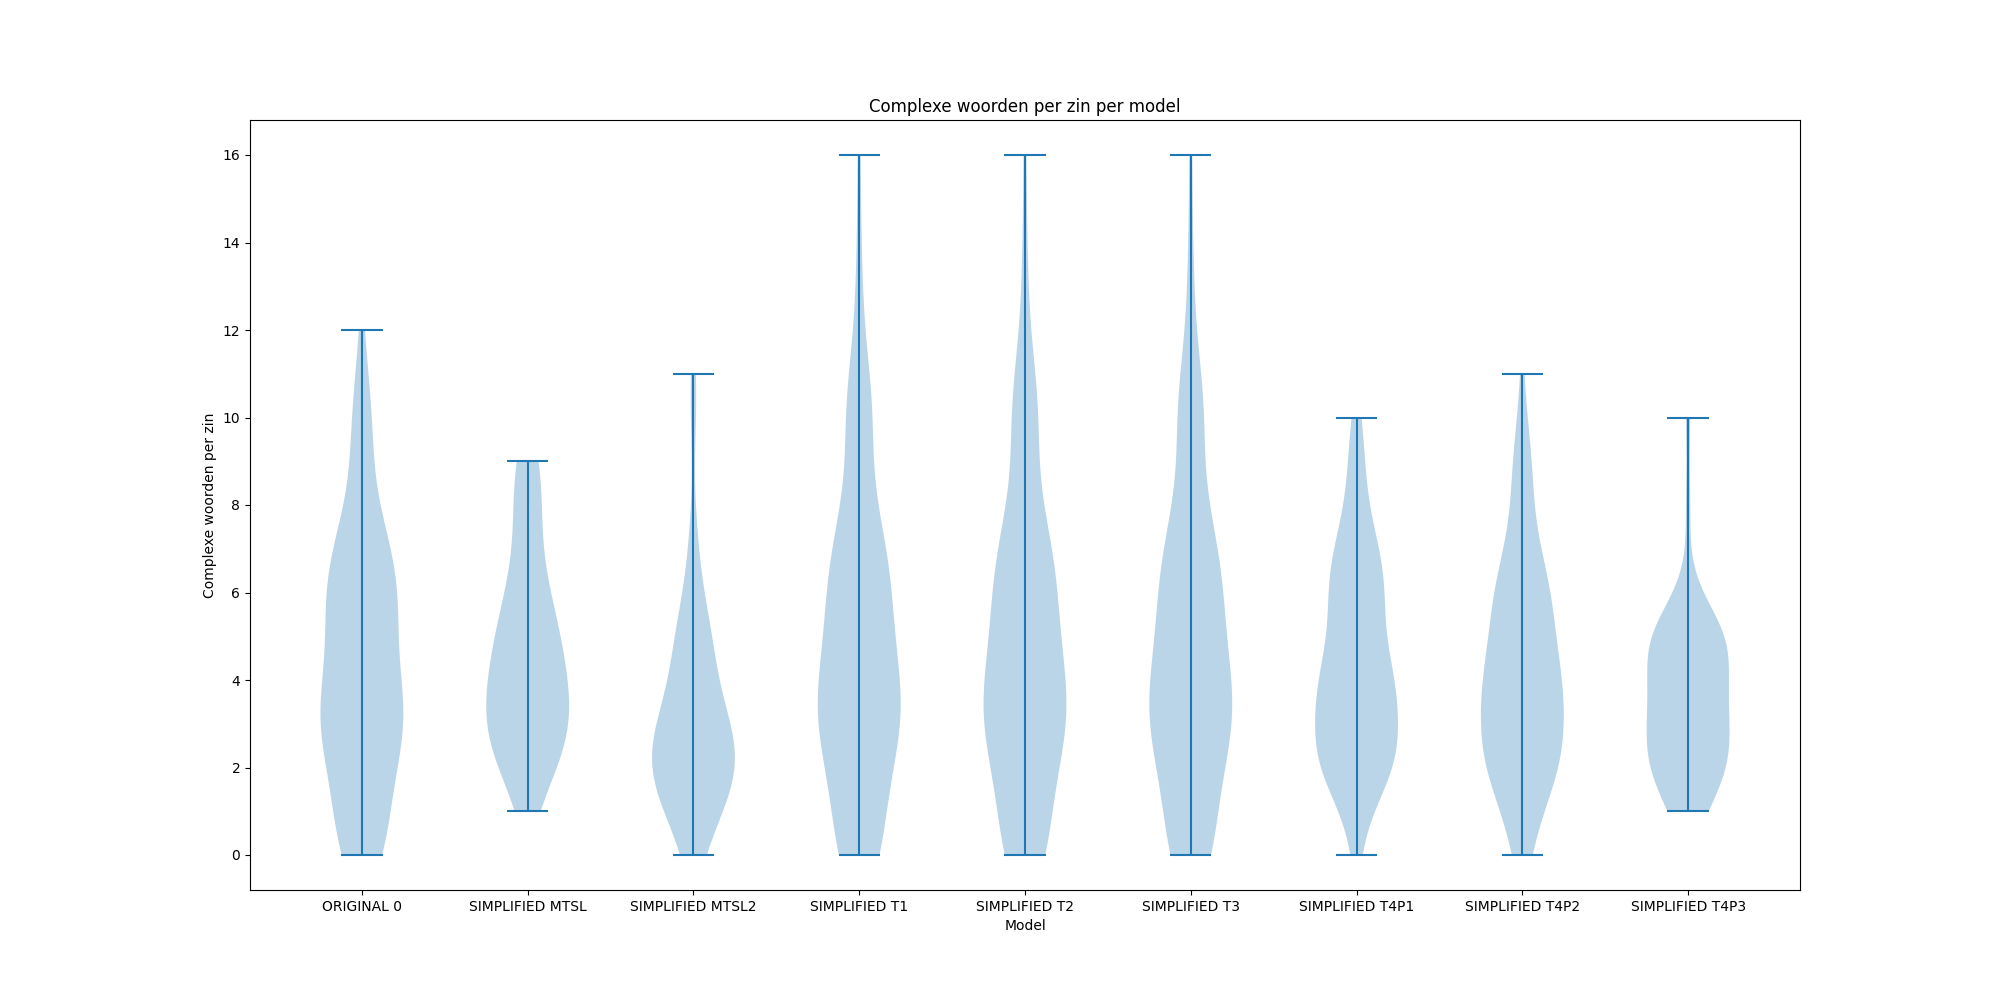
\includegraphics[width=\linewidth]{img/violinplot-complex-a2.png}
	\caption{Gemiddeld aantal complexe woorden per zin gegroepeerd op model voor A2.}
	\label{img:violinplot-complex-a2}
\end{figure}

\begin{figure}
	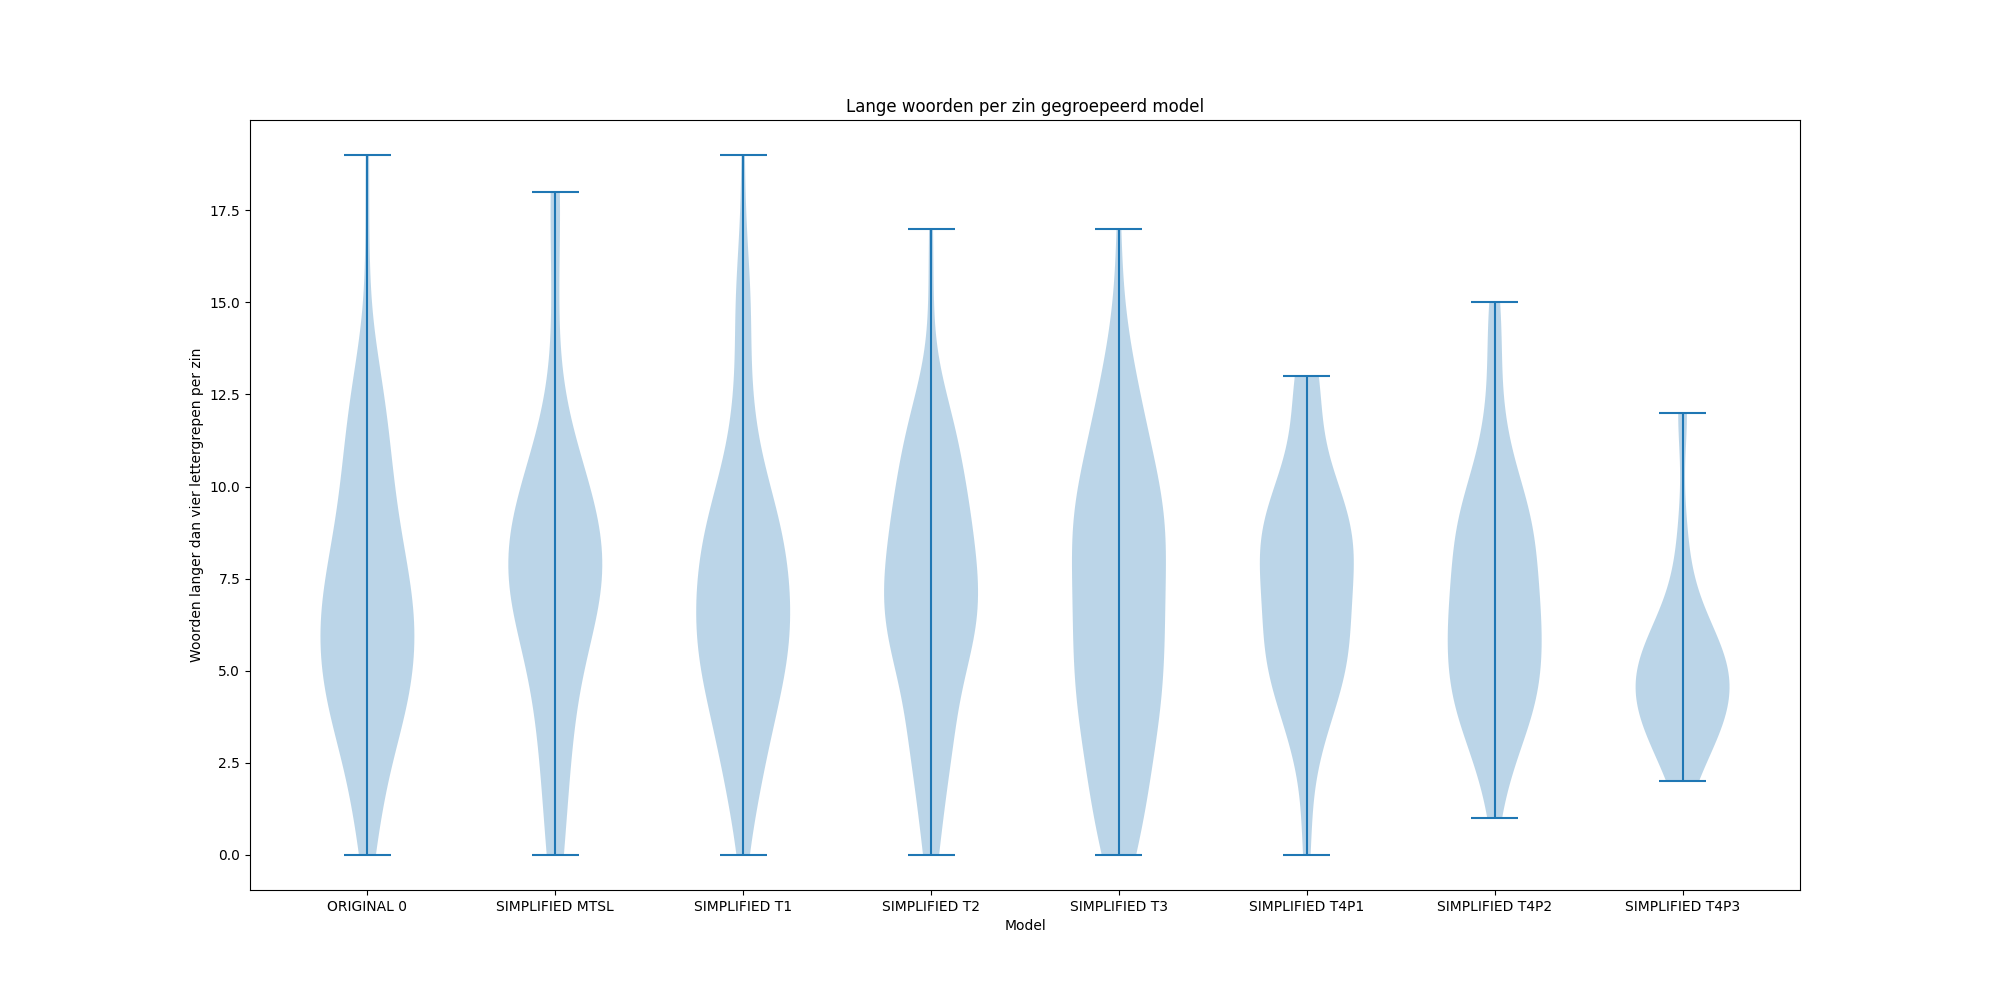
\includegraphics[width=\linewidth]{img/violinplot-long-a1.png}
	\caption{Gemiddeld aantal lange woorden per zin gegroepeerd op model voor A1.}
	\label{img:violinplot-long-a1}
\end{figure}

\begin{figure}
	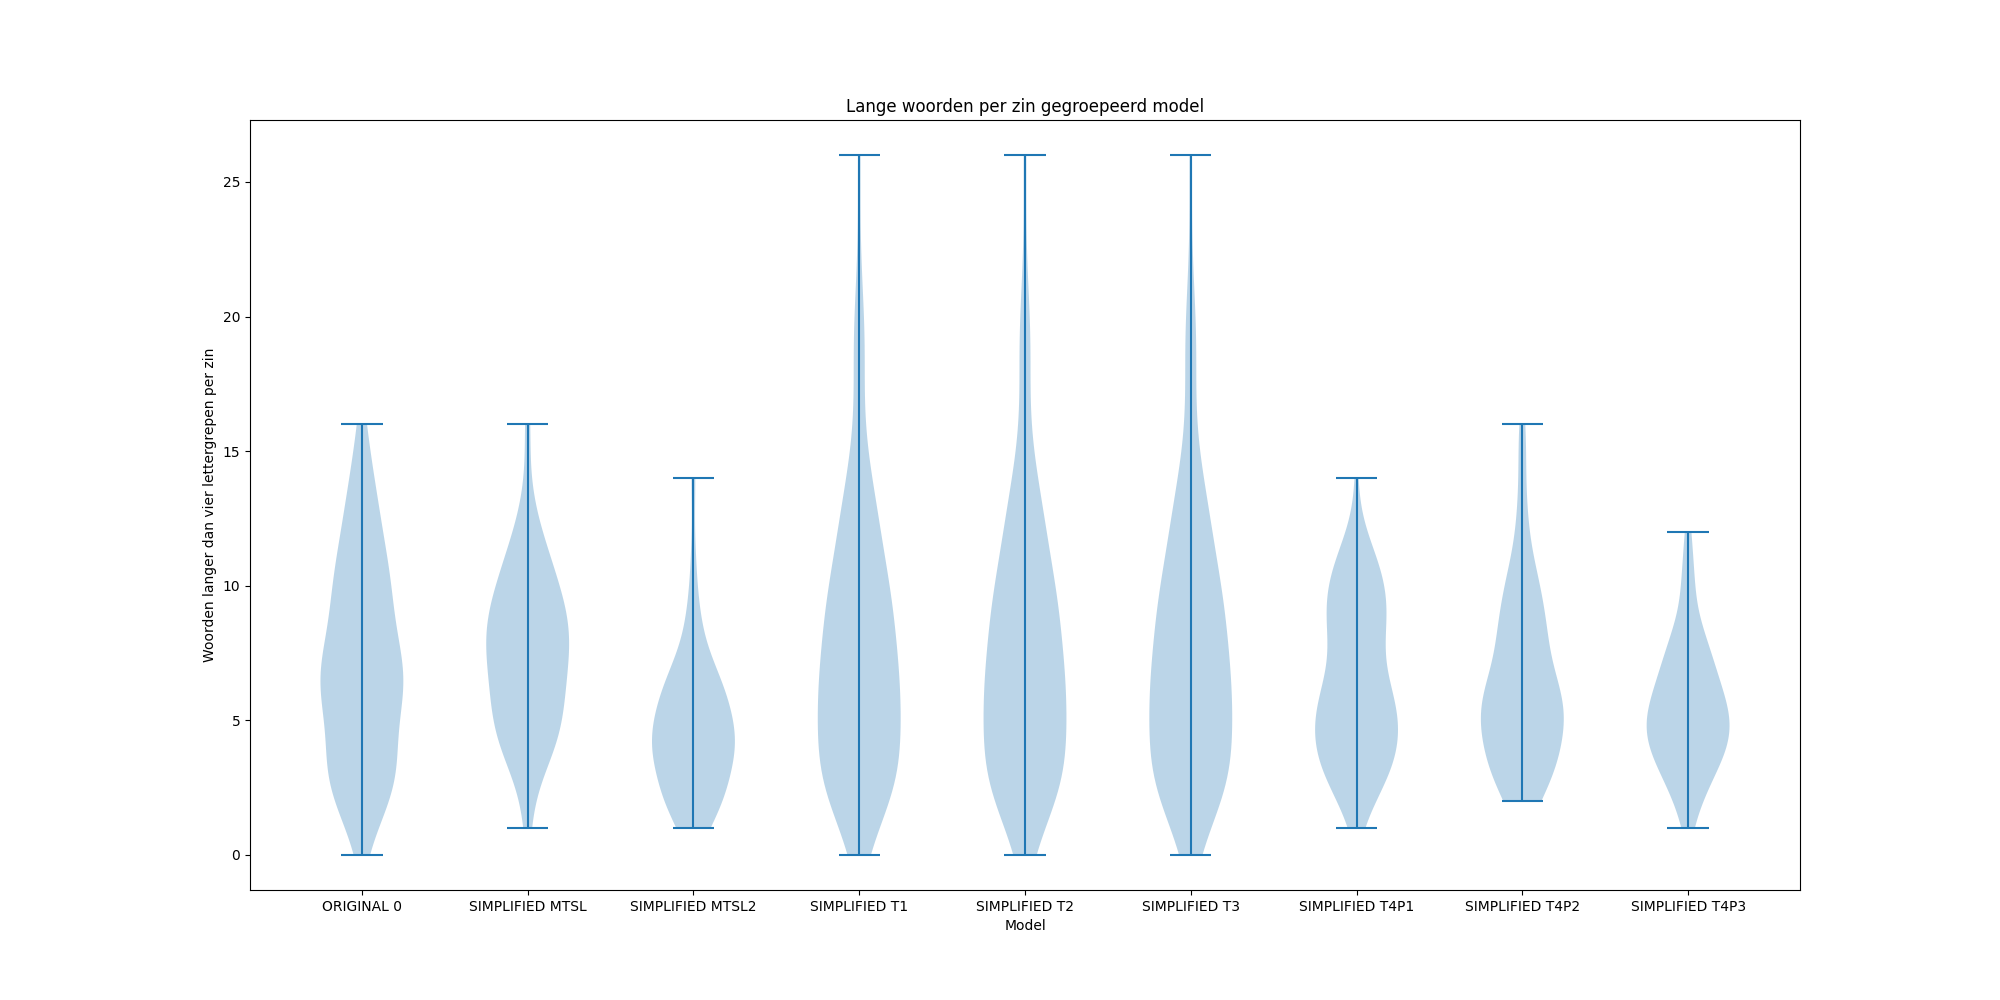
\includegraphics[width=\linewidth]{img/violinplot-long-a2.png}
	\caption{Gemiddeld aantal lange woorden per zin gegroepeerd op model voor A2.}
	\label{img:violinplot-long-a2}
\end{figure}

Ten slotte gebruiken T1, T2 en T3 minder hulpwerkwoorden en vervoegingen van het werkwoord 'zijn'. Daarnaast tonen \ref{img:histplot-aux-a1} en \ref{img:histplot-aux-a2} aan dat alle prompts van T4 een gelijke trend volgen met het aantal vervoegingen en hulpwerkwoorden vergeleken met de MTS-referentieteksten.

\begin{figure}
	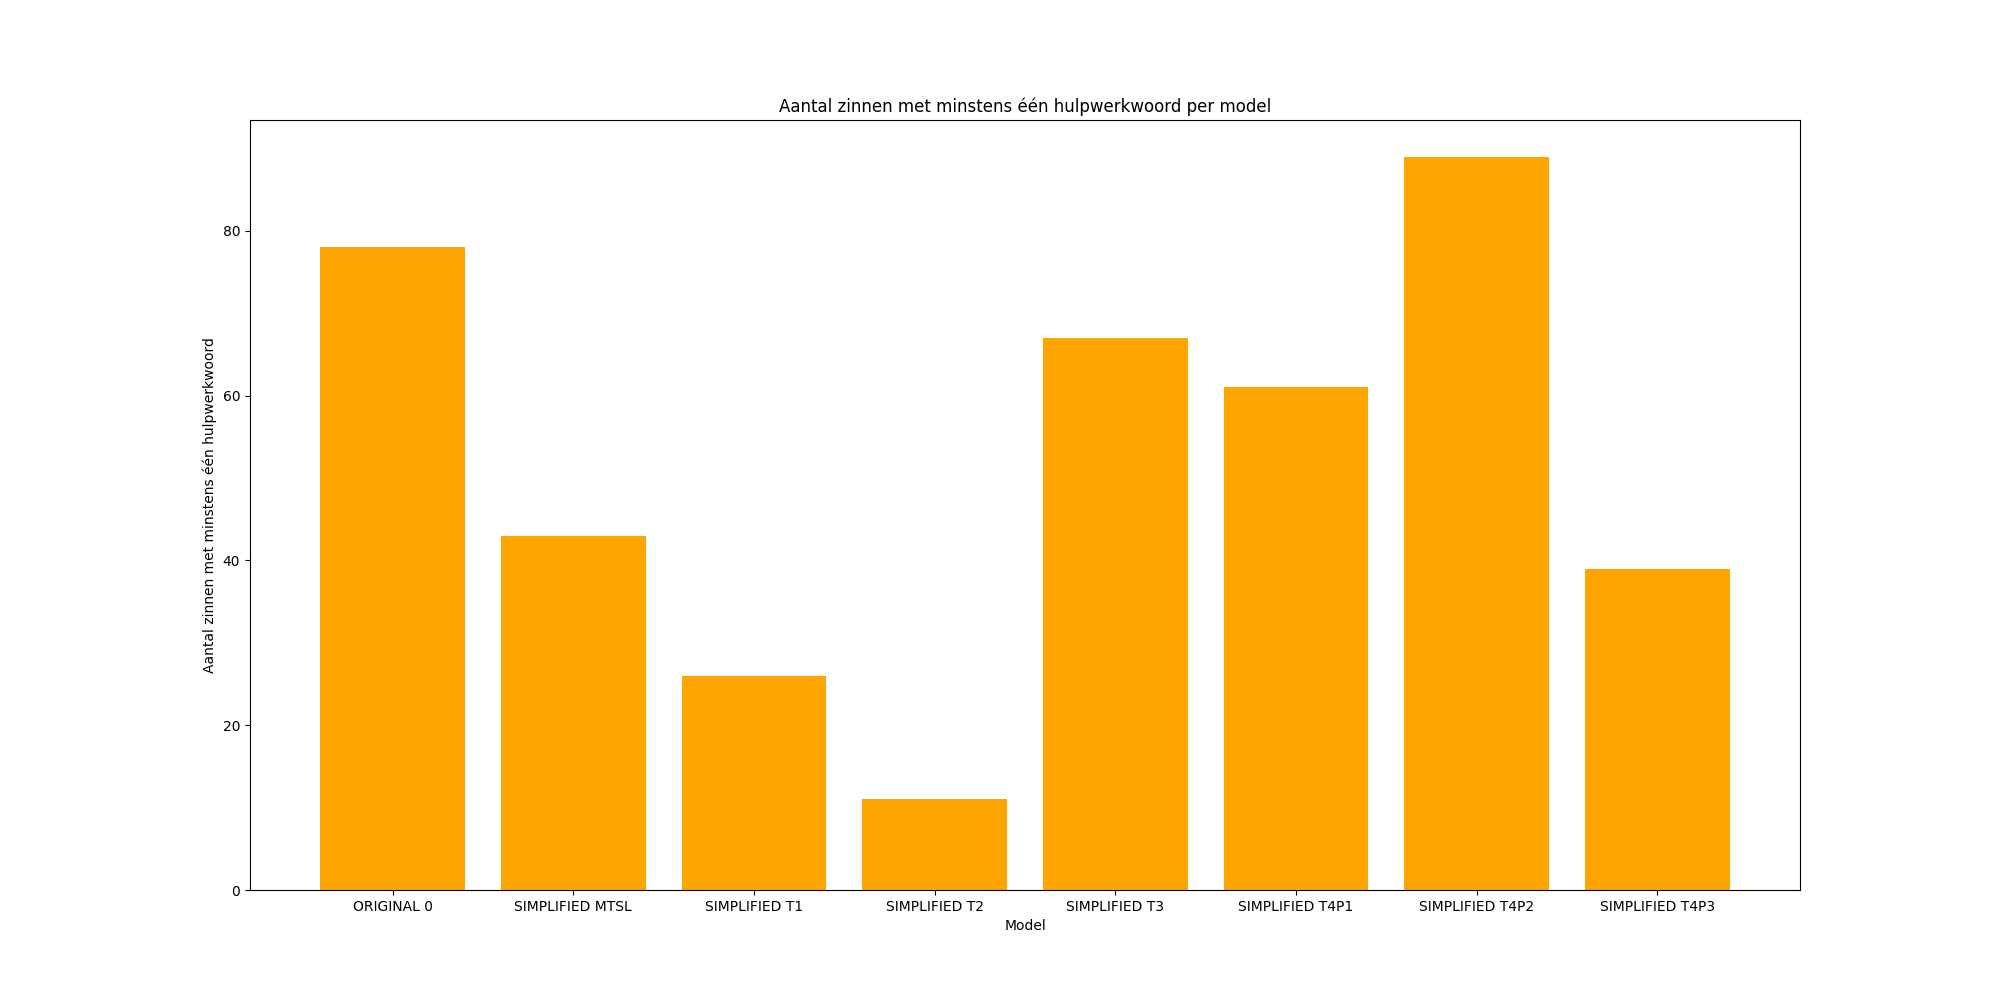
\includegraphics[width=\linewidth]{img/boxplot-aux-a1.png}
	\caption{Gemiddeld aantal hulpwerkwoorden per zin gegroepeerd op model voor A1.}
	\label{img:histplot-aux-a1}
\end{figure}

\begin{figure}
	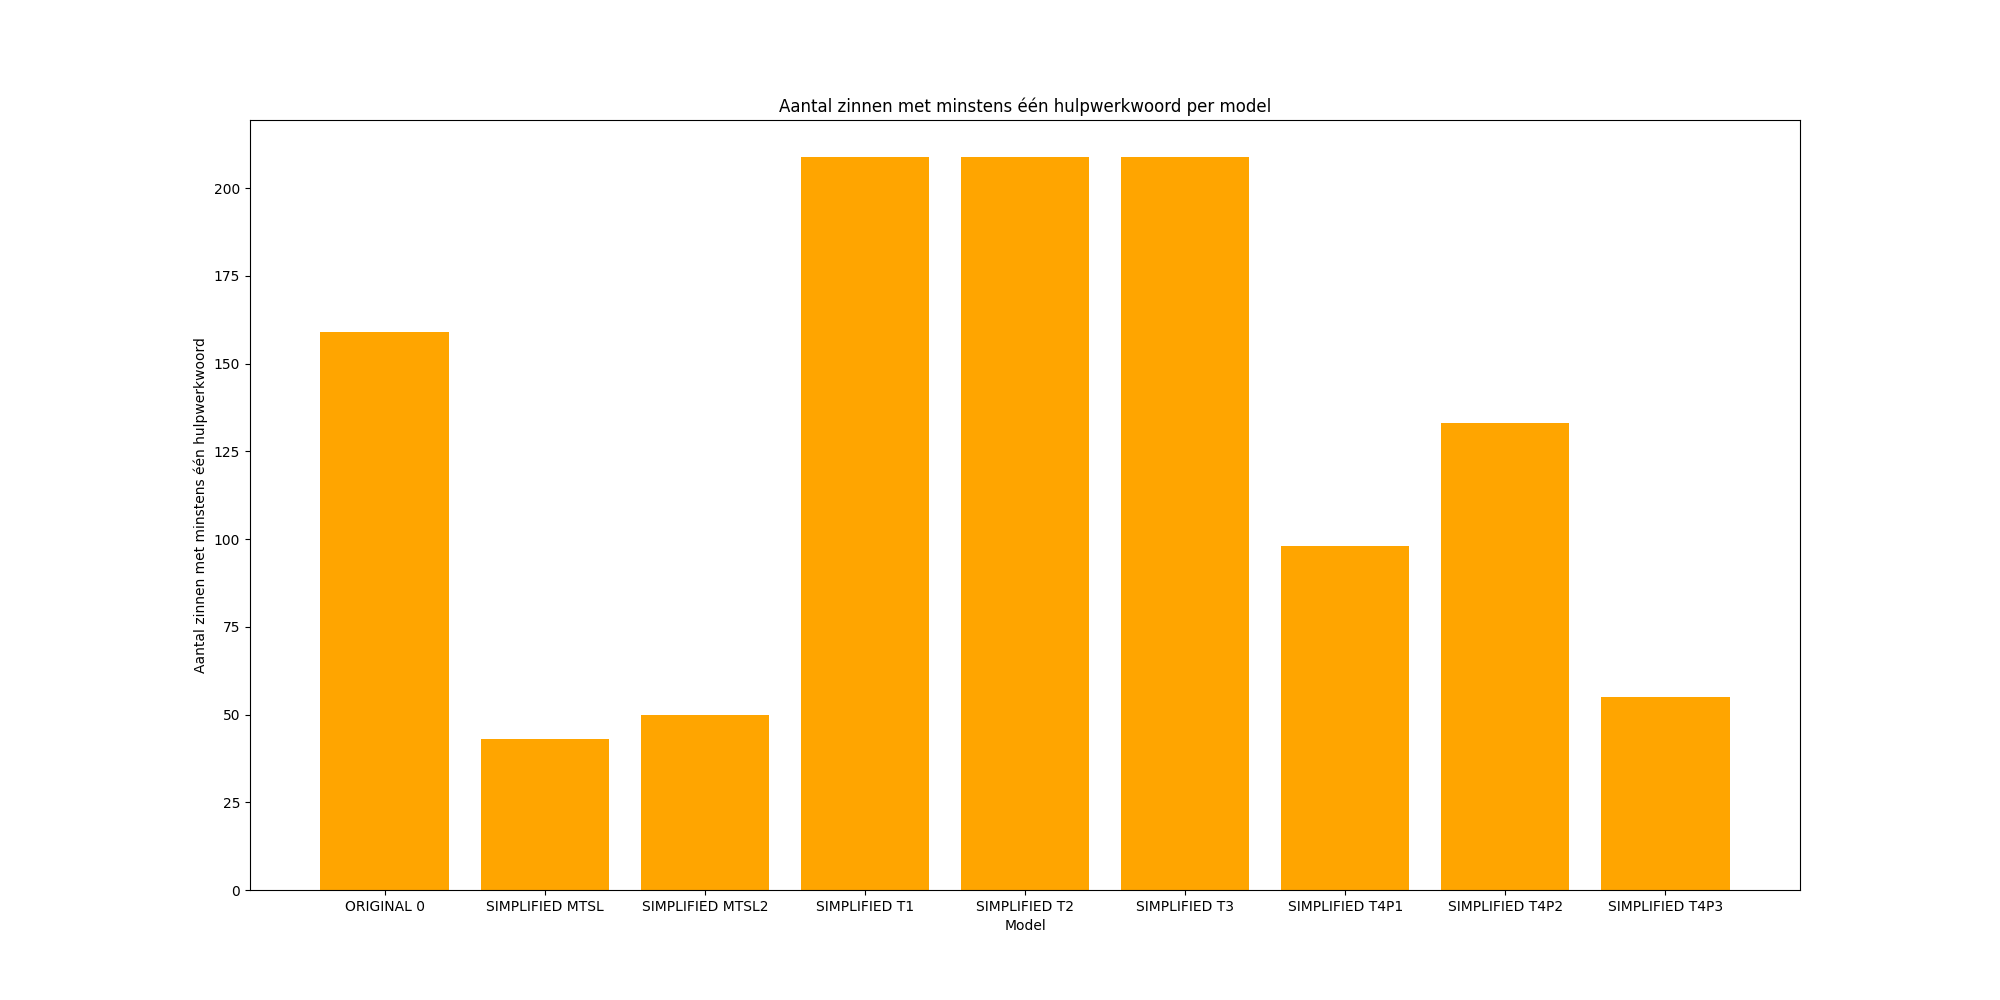
\includegraphics[width=\linewidth]{img/boxplot-aux-a2.png}
	\caption{Gemiddeld aantal hulpwerkwoorden per zin gegroepeerd op model voor A2.}
	\label{img:histplot-aux-a2}
\end{figure}

\begin{figure}
	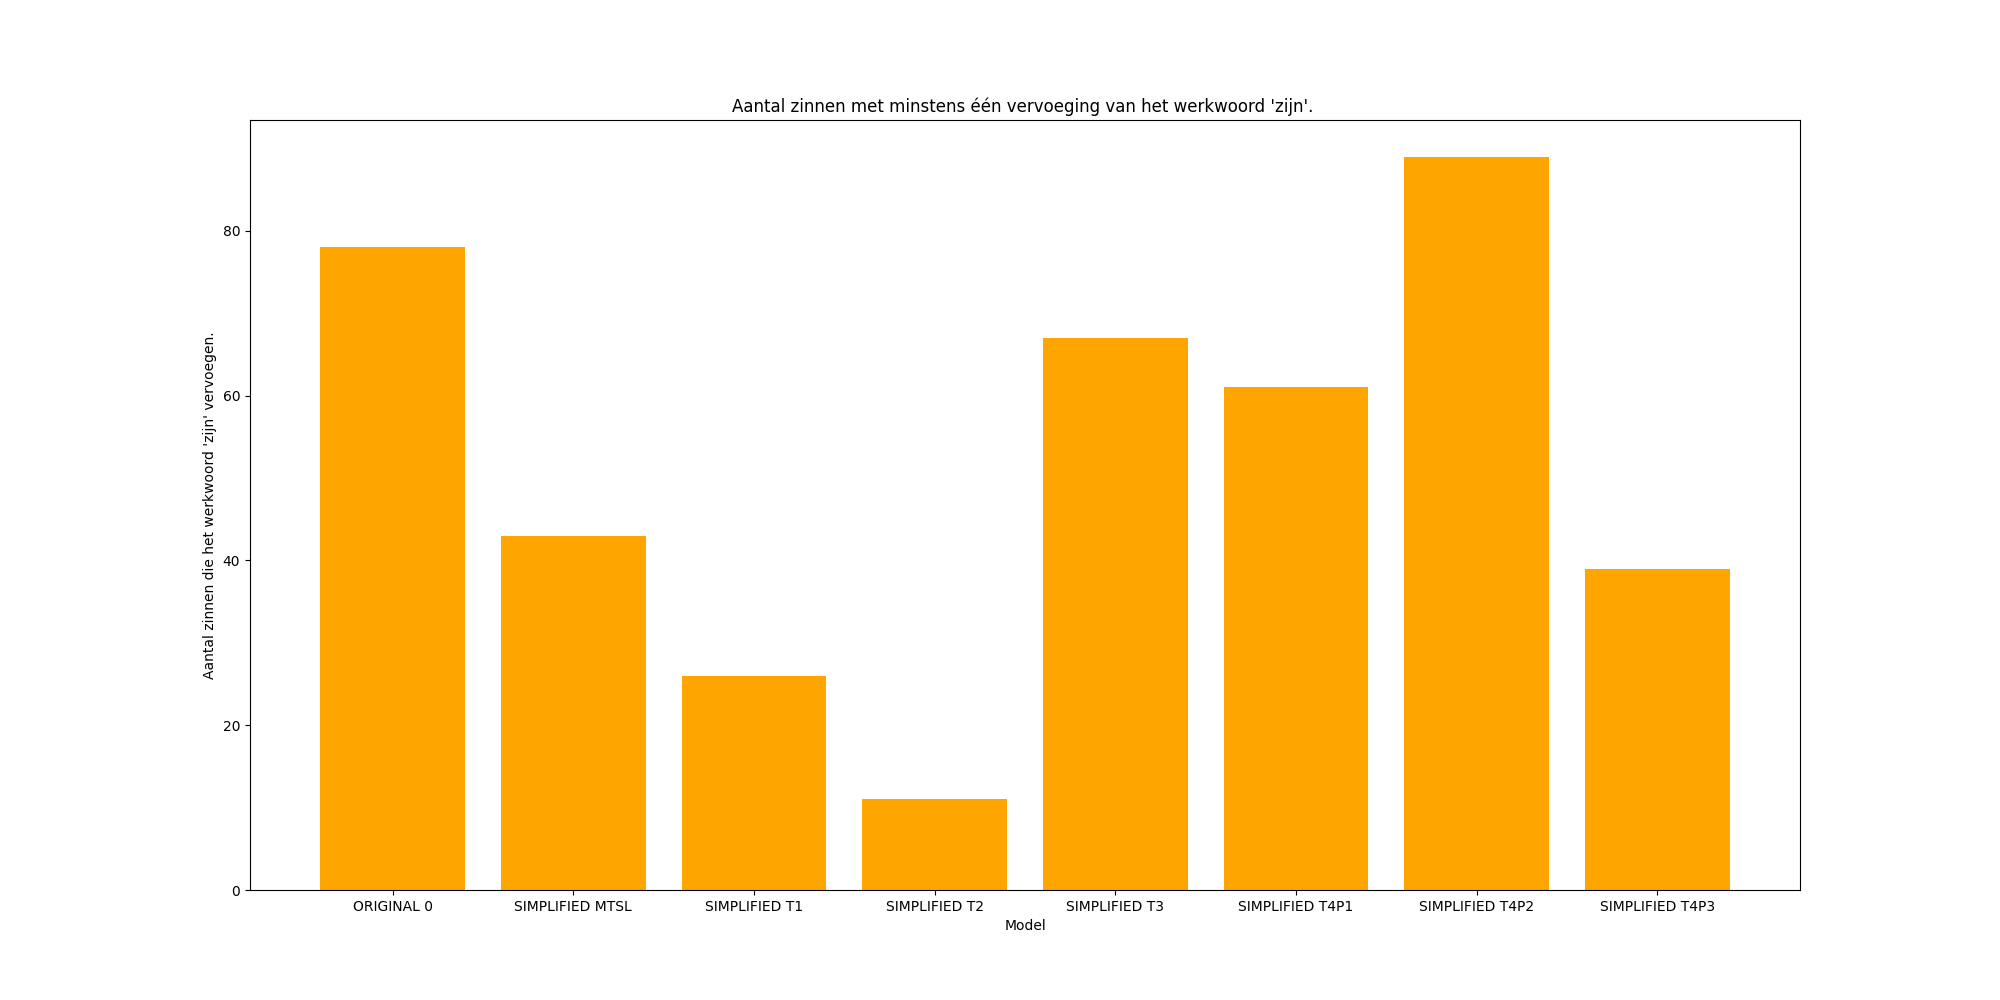
\includegraphics[width=\linewidth]{img/boxplot-tobe-a1.png}
	\caption{Gemiddeld aantal vervoegingen van het werkwoord 'zijn' per zin gegroepeerd op model voor A1.}
	\label{img:histplot-tobe-a1}
\end{figure}

\begin{figure}
	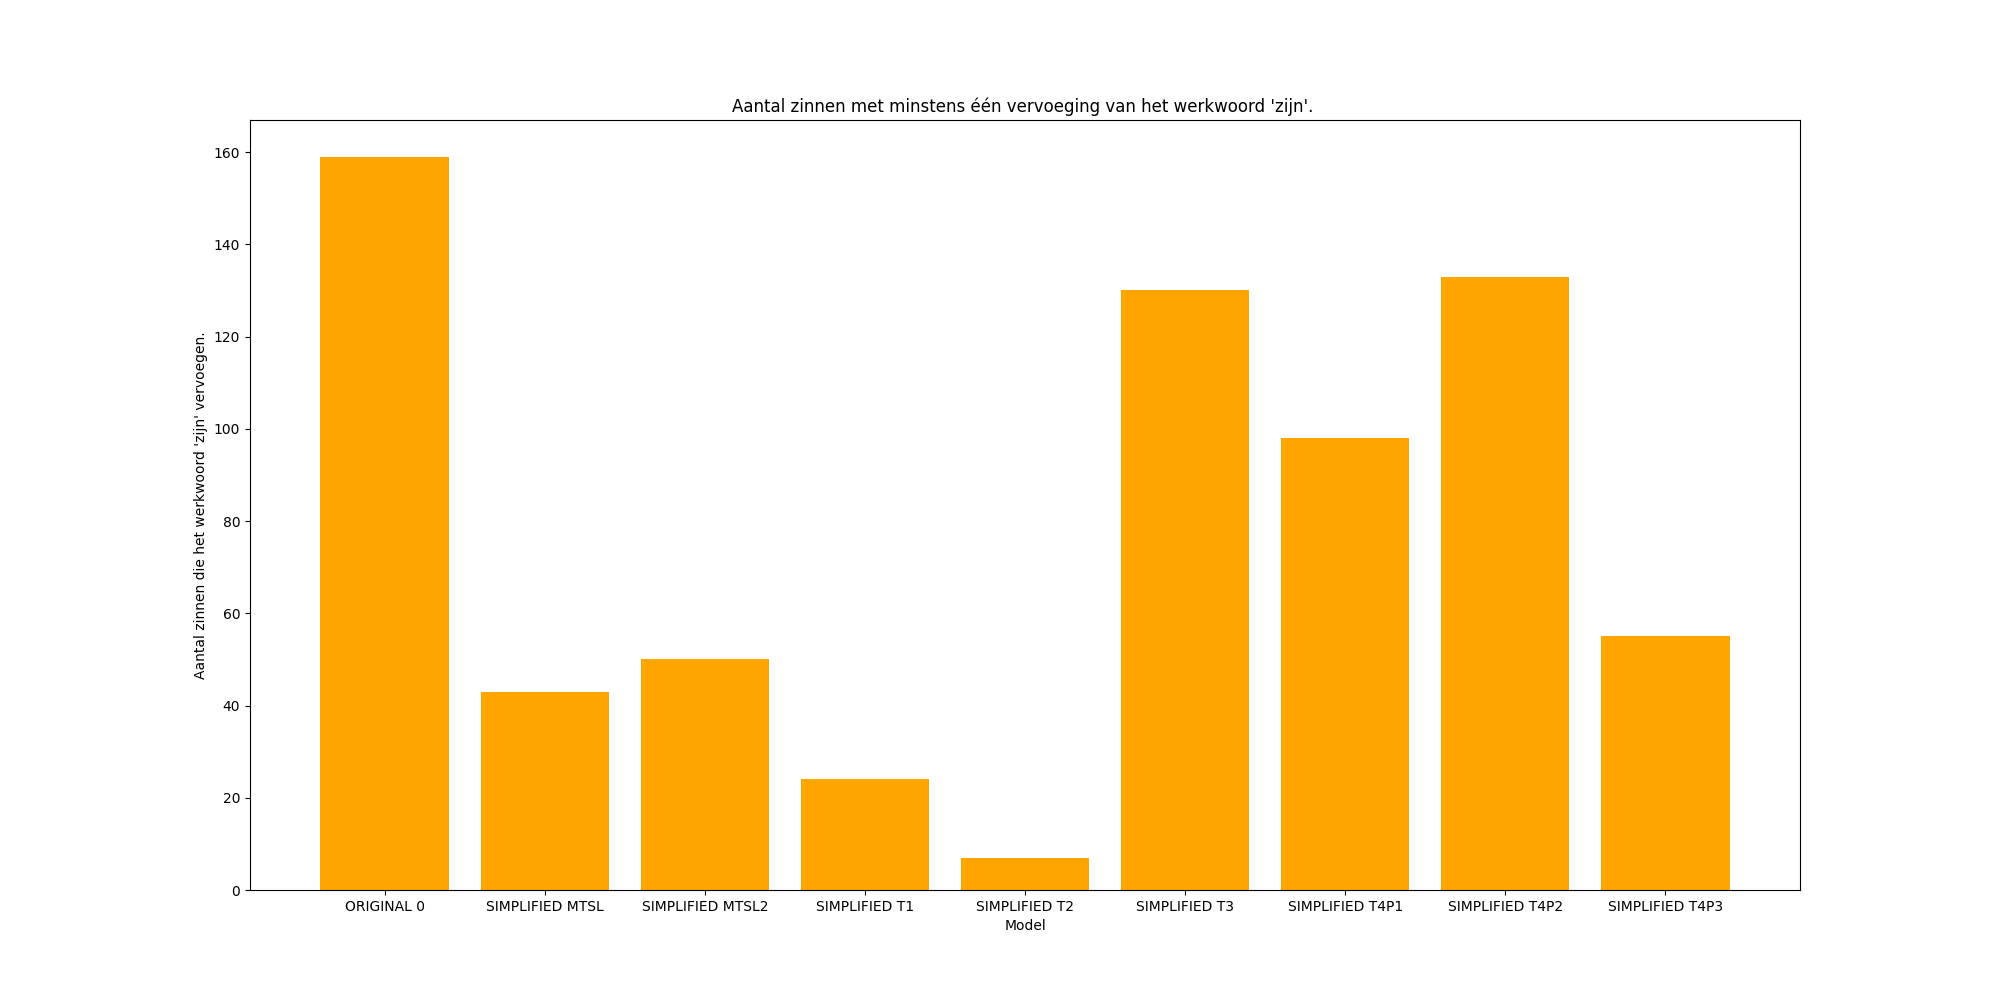
\includegraphics[width=\linewidth]{img/boxplot-tobe-a2.png}
	\caption{Gemiddeld aantal vervoegingen van het werkwoord 'zijn' per zin gegroepeerd op model voor A2.}
	\label{img:histplot-tobe-a2}
\end{figure}

T4P1 en T4P2 vertalen Engelstalige vaktermen naar het Nederlands. Zo blijft de afkorting voor DPKIA intact, maar vertaalt T4P1 hetzelfde woord naar het Nederlands.  T1, T2, T3 en T4P3 houden hier echter geen rekening mee en behouden de oorspronkelijke versie van de tekst. De auteurs schrijven alle afkortingen voluit, zoals beschreven in de richtlijnen.

\medspace

Alle taalmodellen kunnen lexicale vereenvoudiging toepassen. De handmatig vereenvoudigde referentieteksten bevatten zinnen die vakjargon gebruiken op het niveau van 15 tot 18 jarige studenten. T4P1 kan uitleg tussen ronde haakjes schrijven, wanneer het geen eenvoudiger synoniem kan vinden. T4P1, T1, T2 en T3 passen woorden aan, maar schrijven geen extra uitleg. T4P3 past deze techniek minder toe dan de vooraf vermelde taalmodellen.

\medspace

T4P3 verkort lange zinnen door deze op te splitsen. T1, T2 en T3 behalen een gelijke zinslengte als dat van de oorspronkelijke zin. T4P1 en T4P2 kunnen snel langere zinnen genereren, maar smelten geen twee zinnen met elkaar samen.

\medspace

Geen taalmodel wijkt af van de hoofdgedachte van het oorspronkelijke wetenschappelijk artikel. Hoewel T1, T2 en T3 deels afgebroken zinnen kan genereren, bevatten deze zinnen de hoofdgedachte. T2 bevat minder dan 10\% van het oorspronkelijk artikel en ontbreekt daarbij bijzaken die nodig zijn om alle vragen in \ref{ch:referentietekst} te kunnen begrijpen en te beantwoorden. Tenslotte verwerken T1, T2 en T3 de APA- en California bronvermeldingen niet in de vereenvoudigde teksten. Hoewel T4 deze wel verwerkt, bevat de tekst na een vereenvoudiging deze bronvermeldingen niet meer.

\medspace

Ter conclusie scoren de drie prompts van T4 beter op iedere gemeten techniek. Het taalmodel en de verwante drie prompts genereren coherente teksten met een verlaagde lexicale complexiteit. Echter houden de geteste taalmodellen weinig tot geen rekening met afkortingen of bronvermeldingen.

\section{Het prototype voor tekstvereenvoudiging met ATS vergeleken met top-of-the-line tools.}

% deelvraag: Hoe kan een intuïtieve en lokale webtoepassing worden ontwikkeld die zowel scholieren met dyslexie als docenten helpt bij het vereenvoudigen van wetenschappelijke artikelen met behoud van semantiek, jargon en zinsstructuren?

Gebruikers kunnen vanuit de homepagina drie schermen kiezen: het lerarencomponent, het scholierencomponent en een instellingenpagina. In de instellingenpagina kunnen eindgebruikers de opmaakopties aanpassen naargelang hun keuze. Figuur \ref{img:website-instellingen} toont alle aanpasbare opmaakopties 

\begin{center}
	\begin{figure}[H]
		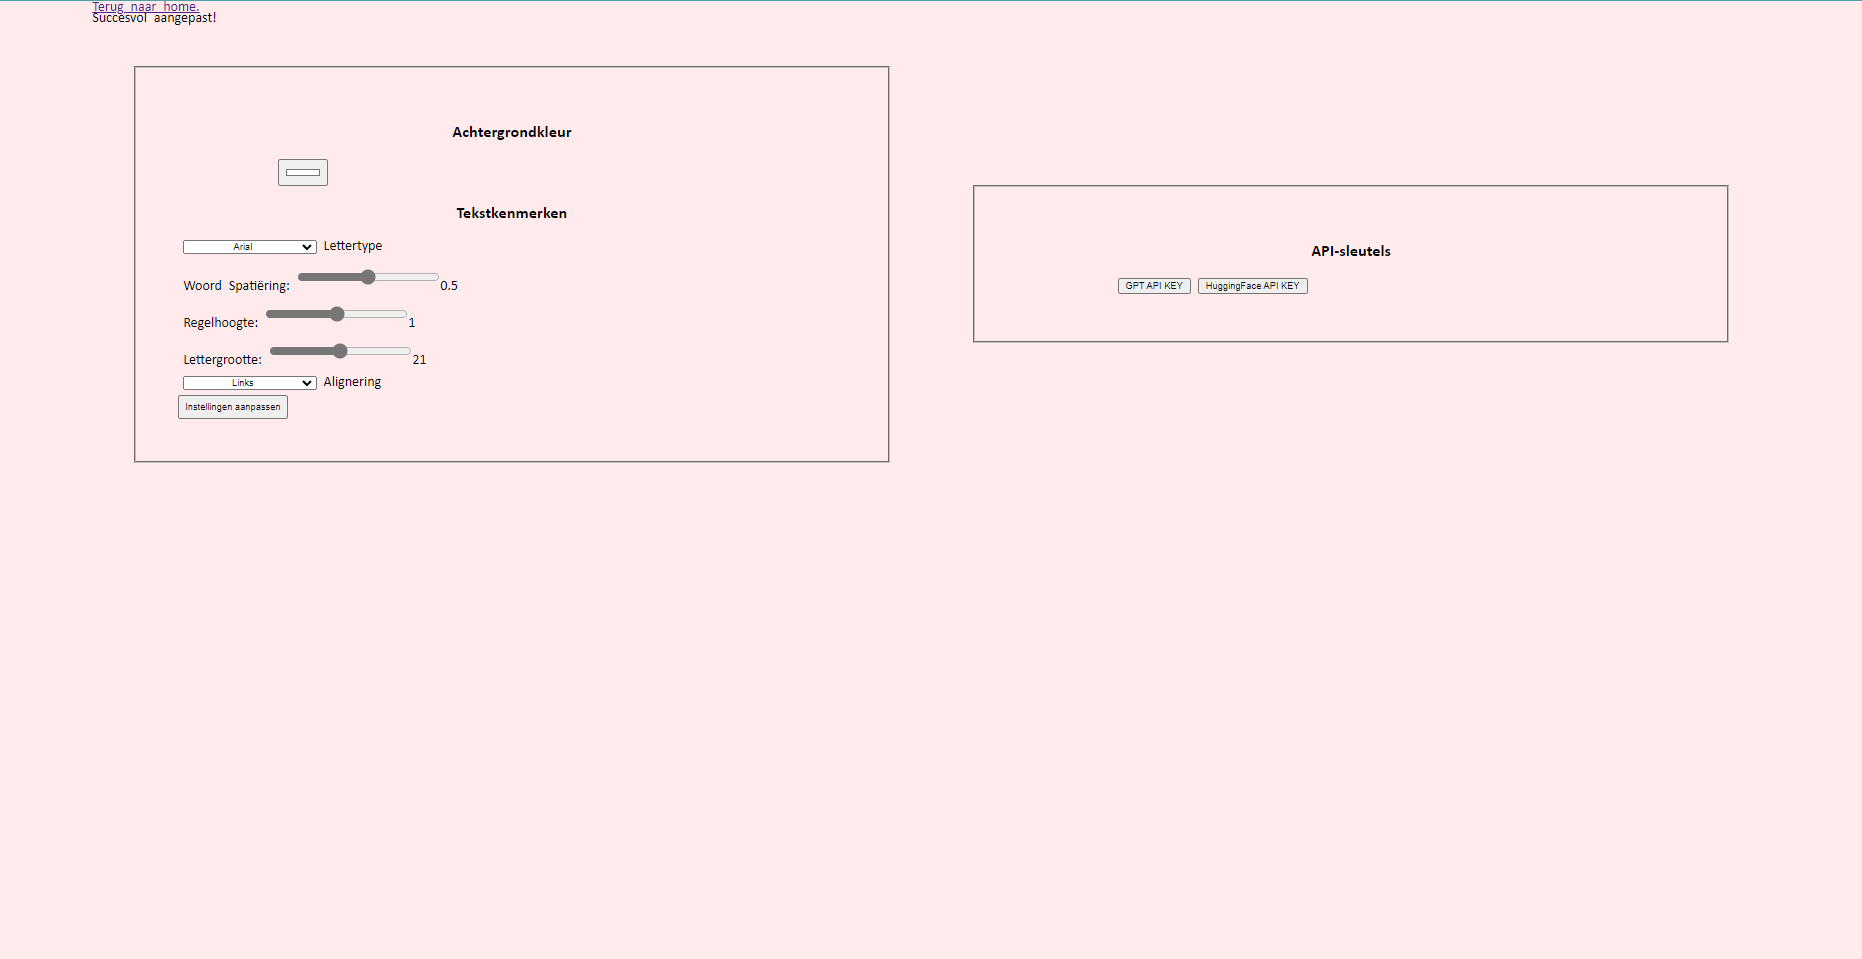
\includegraphics[width=\linewidth]{img/website-instellingen.png}
		\caption{Voorbeeldweergave van de instellingenpagina.}
		\label{img:website-instellingen}
	\end{figure}
\end{center}

Bovendien stelt het prototype gebruikers in staat om op basis van gekregen parameters automatisch personaliseerbare pdf en docx-documenten te genereren.

\begin{figure}
	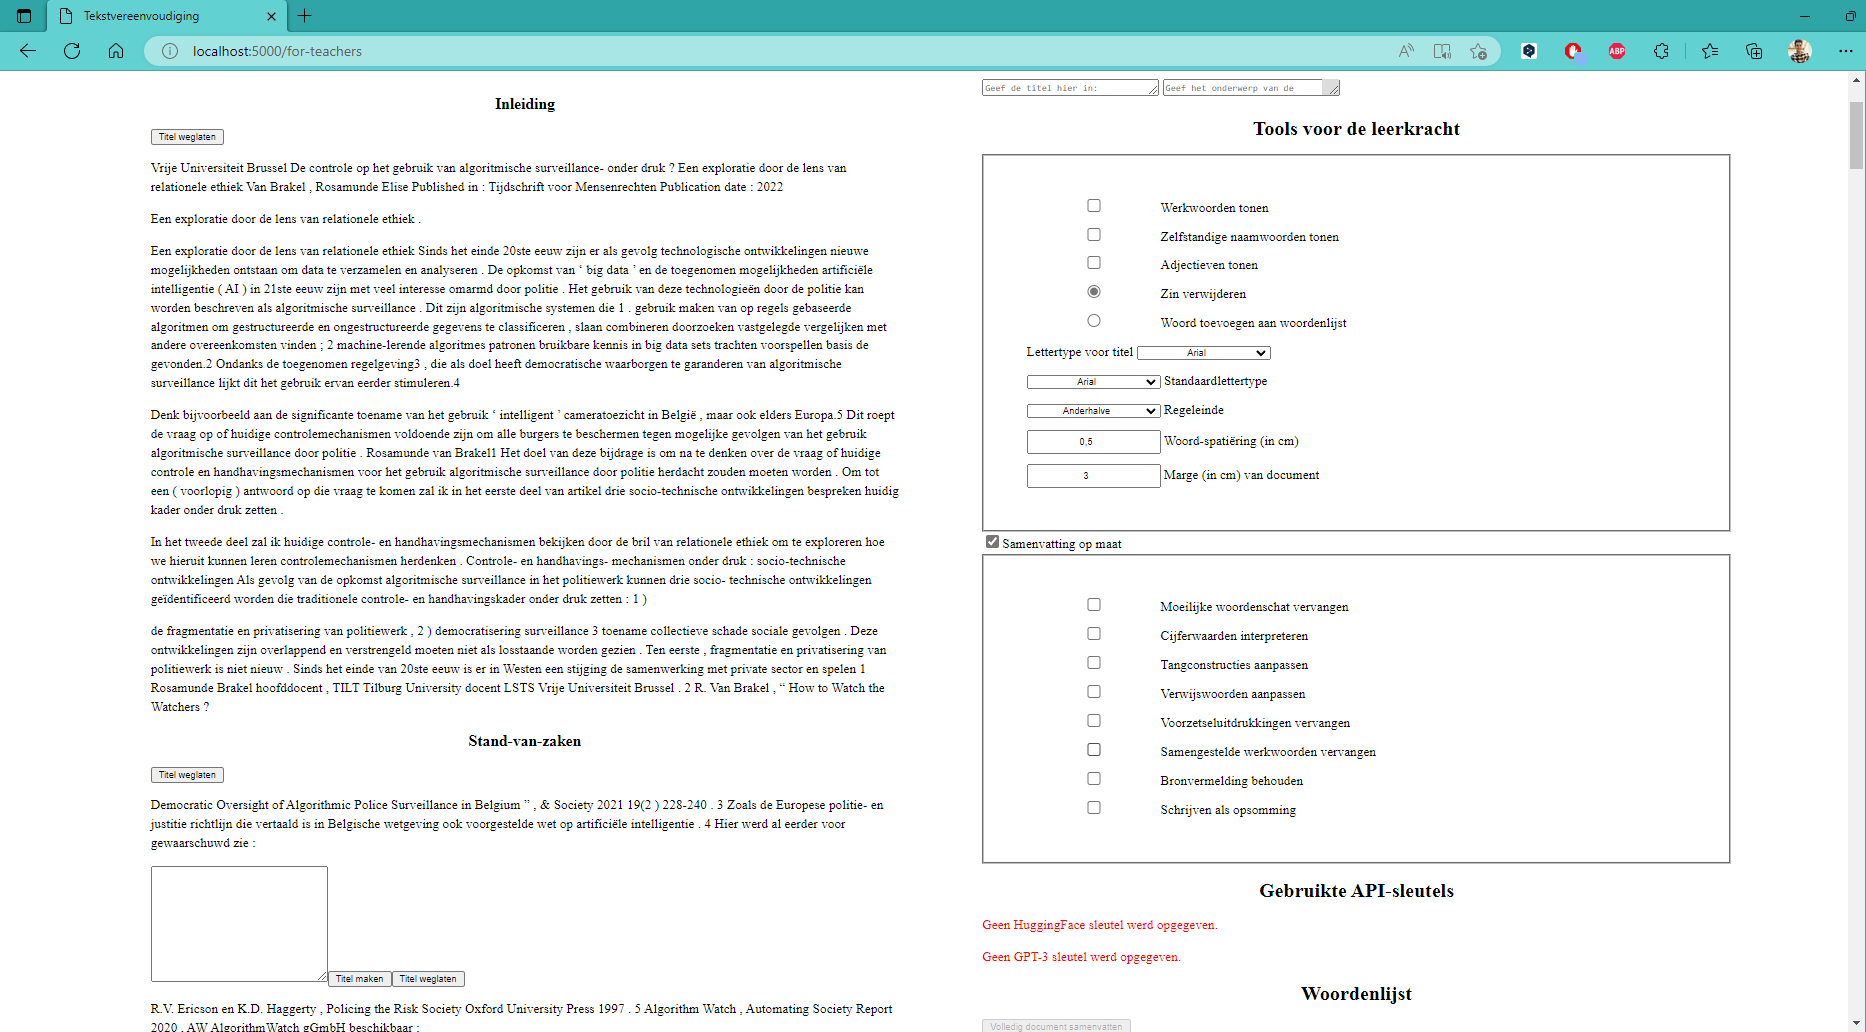
\includegraphics[width=\linewidth]{img/proto-lerarencomponent.png}
	\caption{Een mogelijke weergave van het lerarencomponent met het wetenschappelijk artikel van \textcite{VanBrakel2022} als input.}
	\label{img:proto-lerarencomponent}
\end{figure}

\begin{center}
	\begin{figure}[H]
		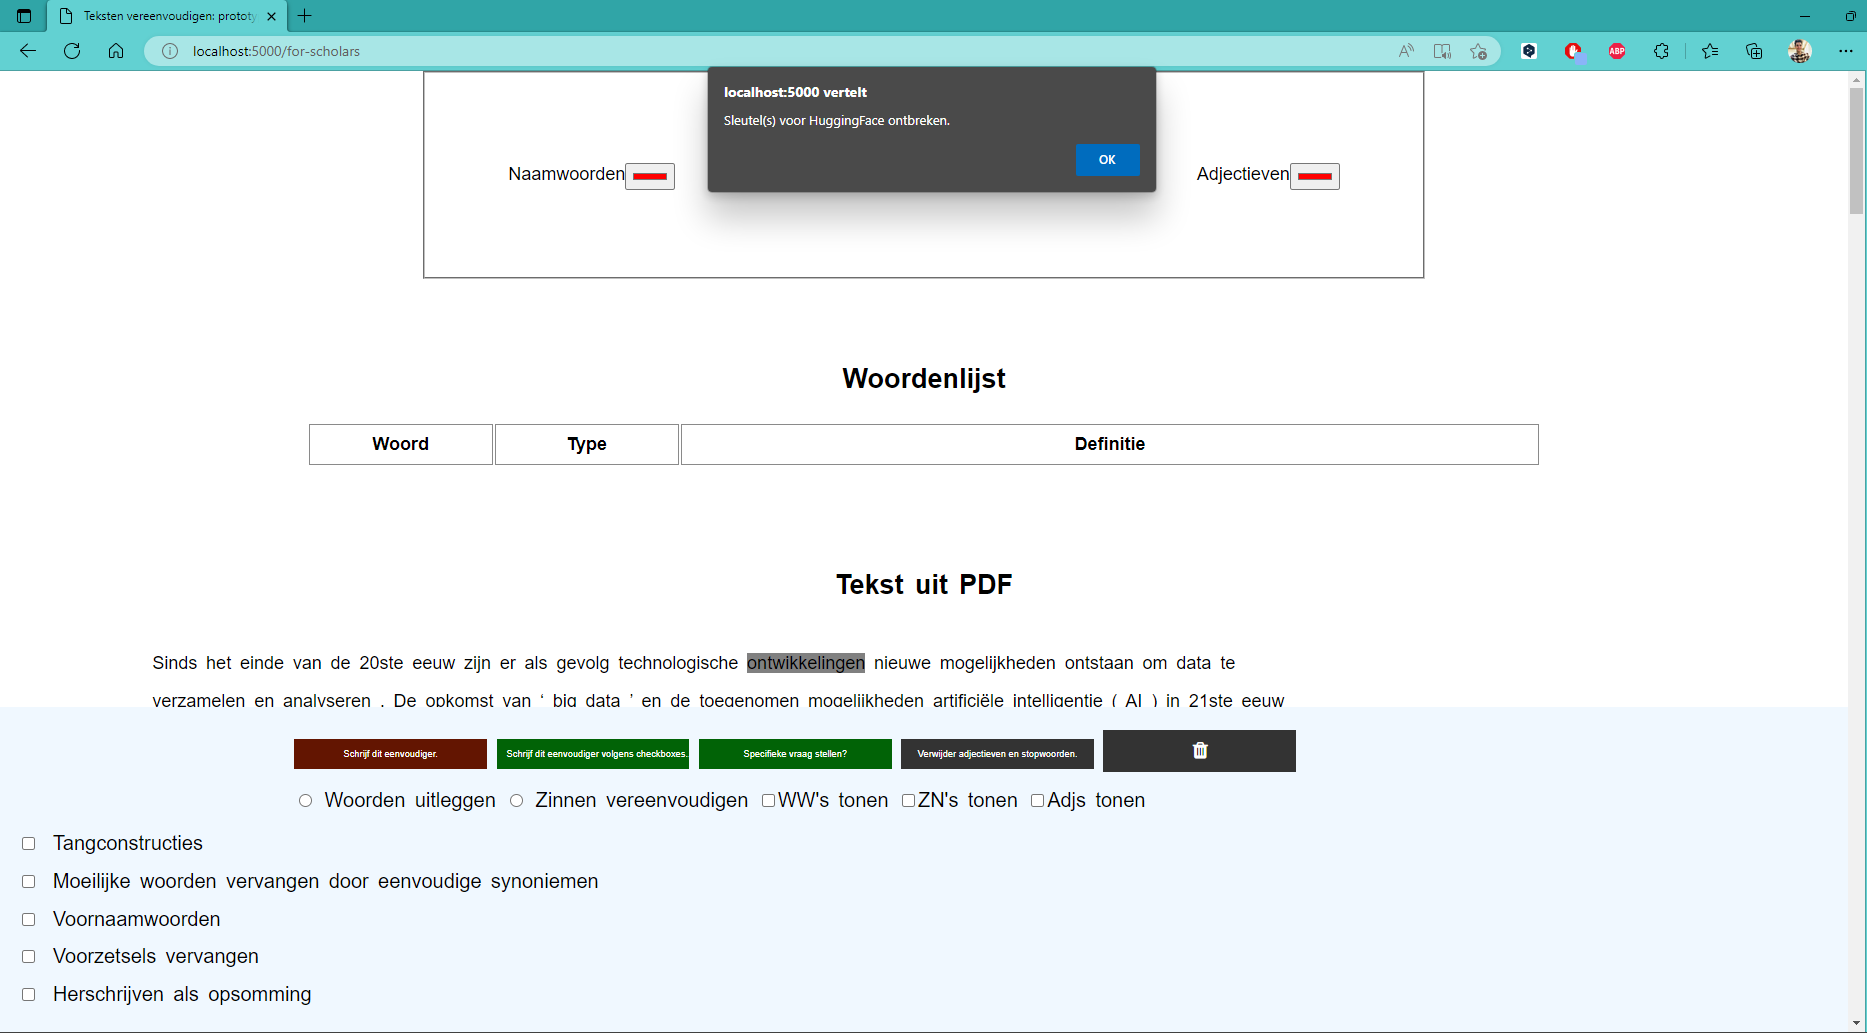
\includegraphics[width=\linewidth]{img/proto-melding.png}
		\caption{Een voorbeeldweergave van het scholierencomponent.}
		\label{img:proto-homescreen-scholieren}
	\end{figure}
\end{center}

Figuur \ref{img:proto-pos-tagging-scholieren} toont een voorbeeldweergave van deze functionaliteit. 

\begin{center}
	\begin{figure}[H]
		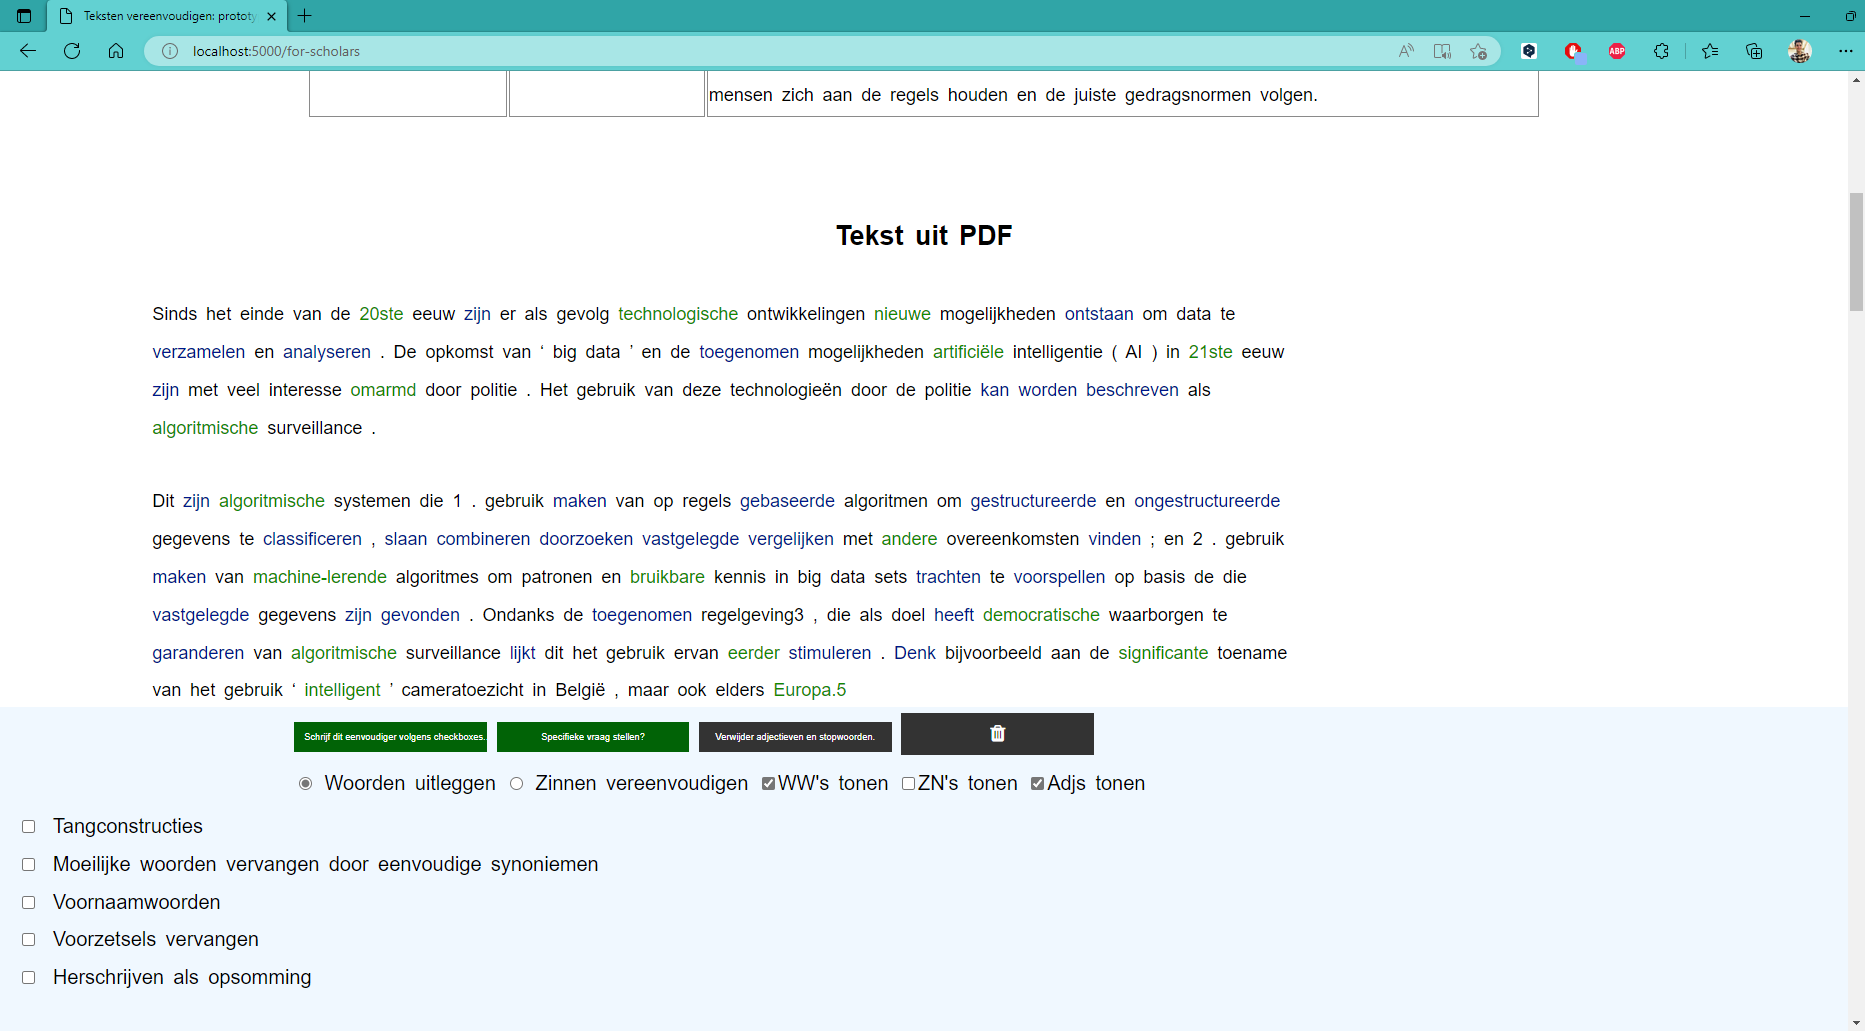
\includegraphics[width=\linewidth]{img/proto-pos-tagging.png}
		\caption{Een voorbeeldweergave van de toepassing van PoS-tagging bij het scholierencomponent.}
		\label{img:proto-pos-tagging-scholieren}
	\end{figure}
\end{center}

Scholieren kunnen zinnen selecteren om daarna deze tekst te laten vereenvoudigen met gepersonaliseerde ATS. Figuren \ref{img:proto-scholieren-step-1} en \ref{img:proto-scholieren-step-3} tonen hoe een gebruiker van gemarkeerde doorlopende tekst een opsomming kan maken met het prototype. Het prototype kan doorlopende tekst omvormen naar een opsomming van tekst. Echter beschikt het prototype geen functionaliteit om doorlopende tekst naar een tabel om te vormen.

\begin{center}
	\begin{figure}[H]
		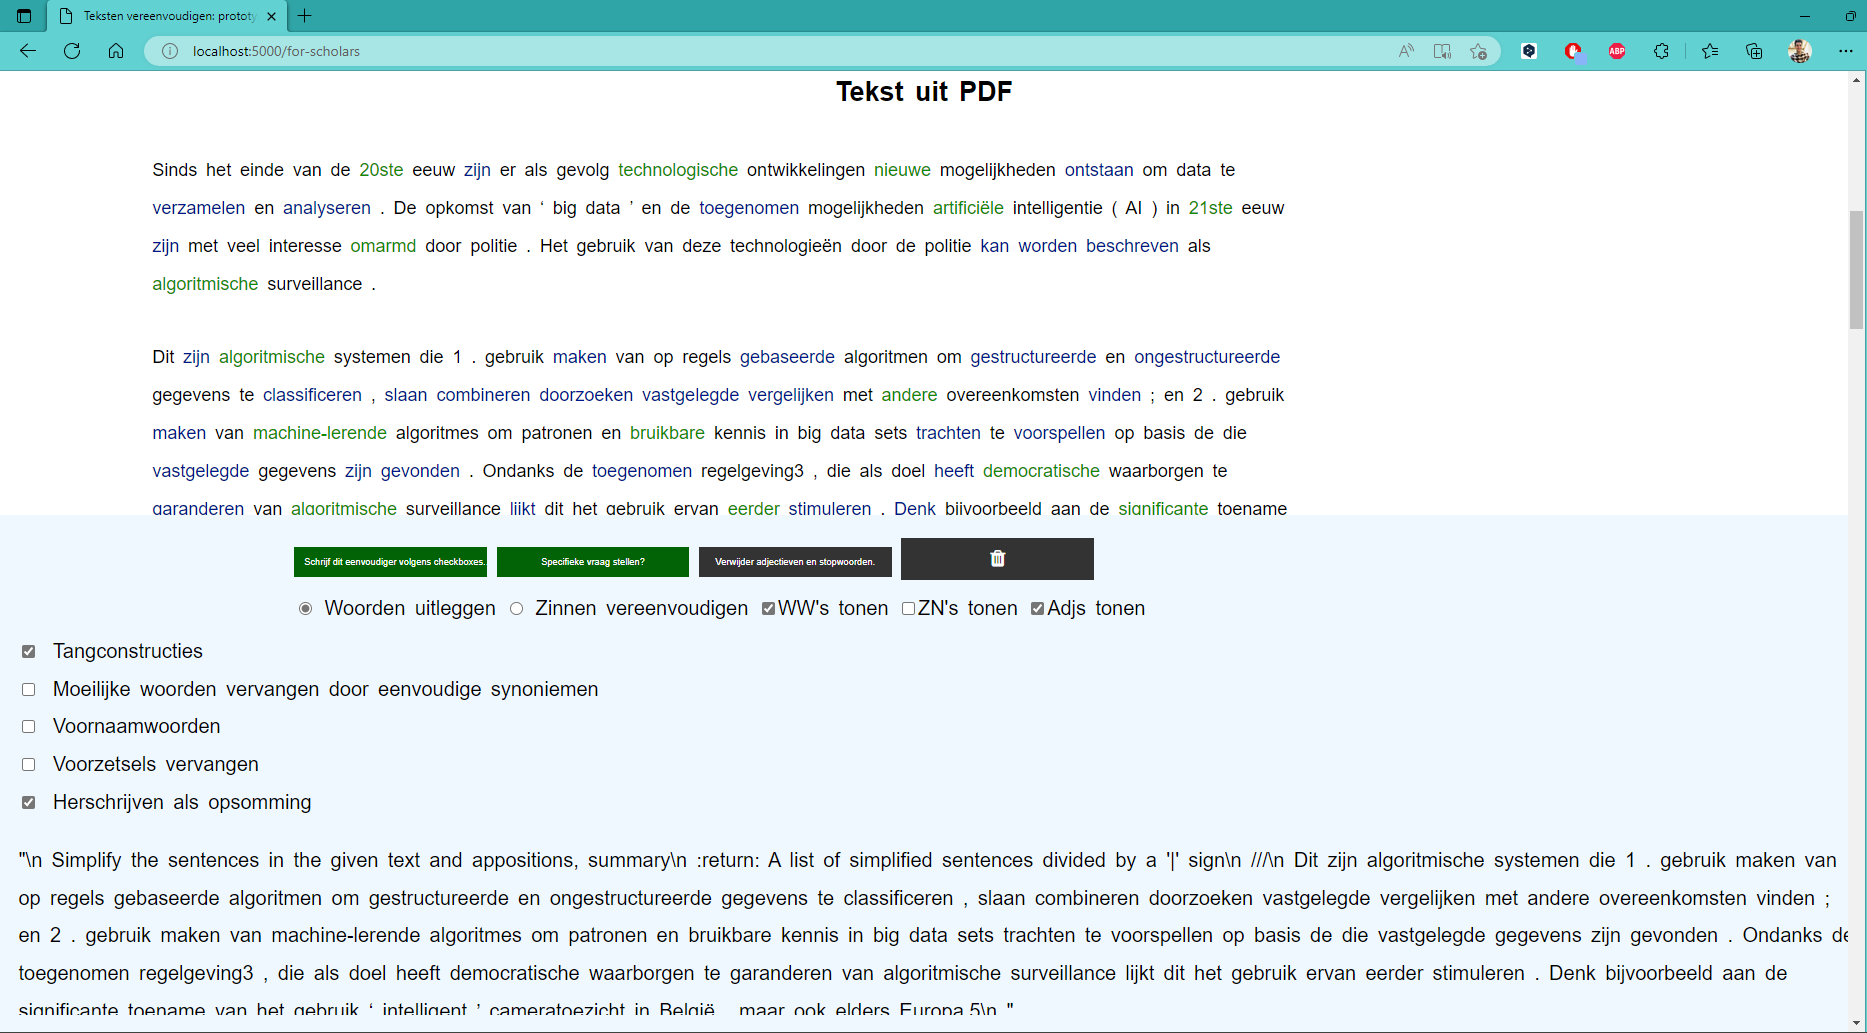
\includegraphics[width=\linewidth]{img/proto-opsomming-1.png}
		\caption{Stap 1 van een gepersonaliseerde tekstvereenvoudiging in het scholierencomponent.}
		\label{img:proto-scholieren-step-1}
	\end{figure}
\end{center}

\begin{center}
	\begin{figure}[H]
		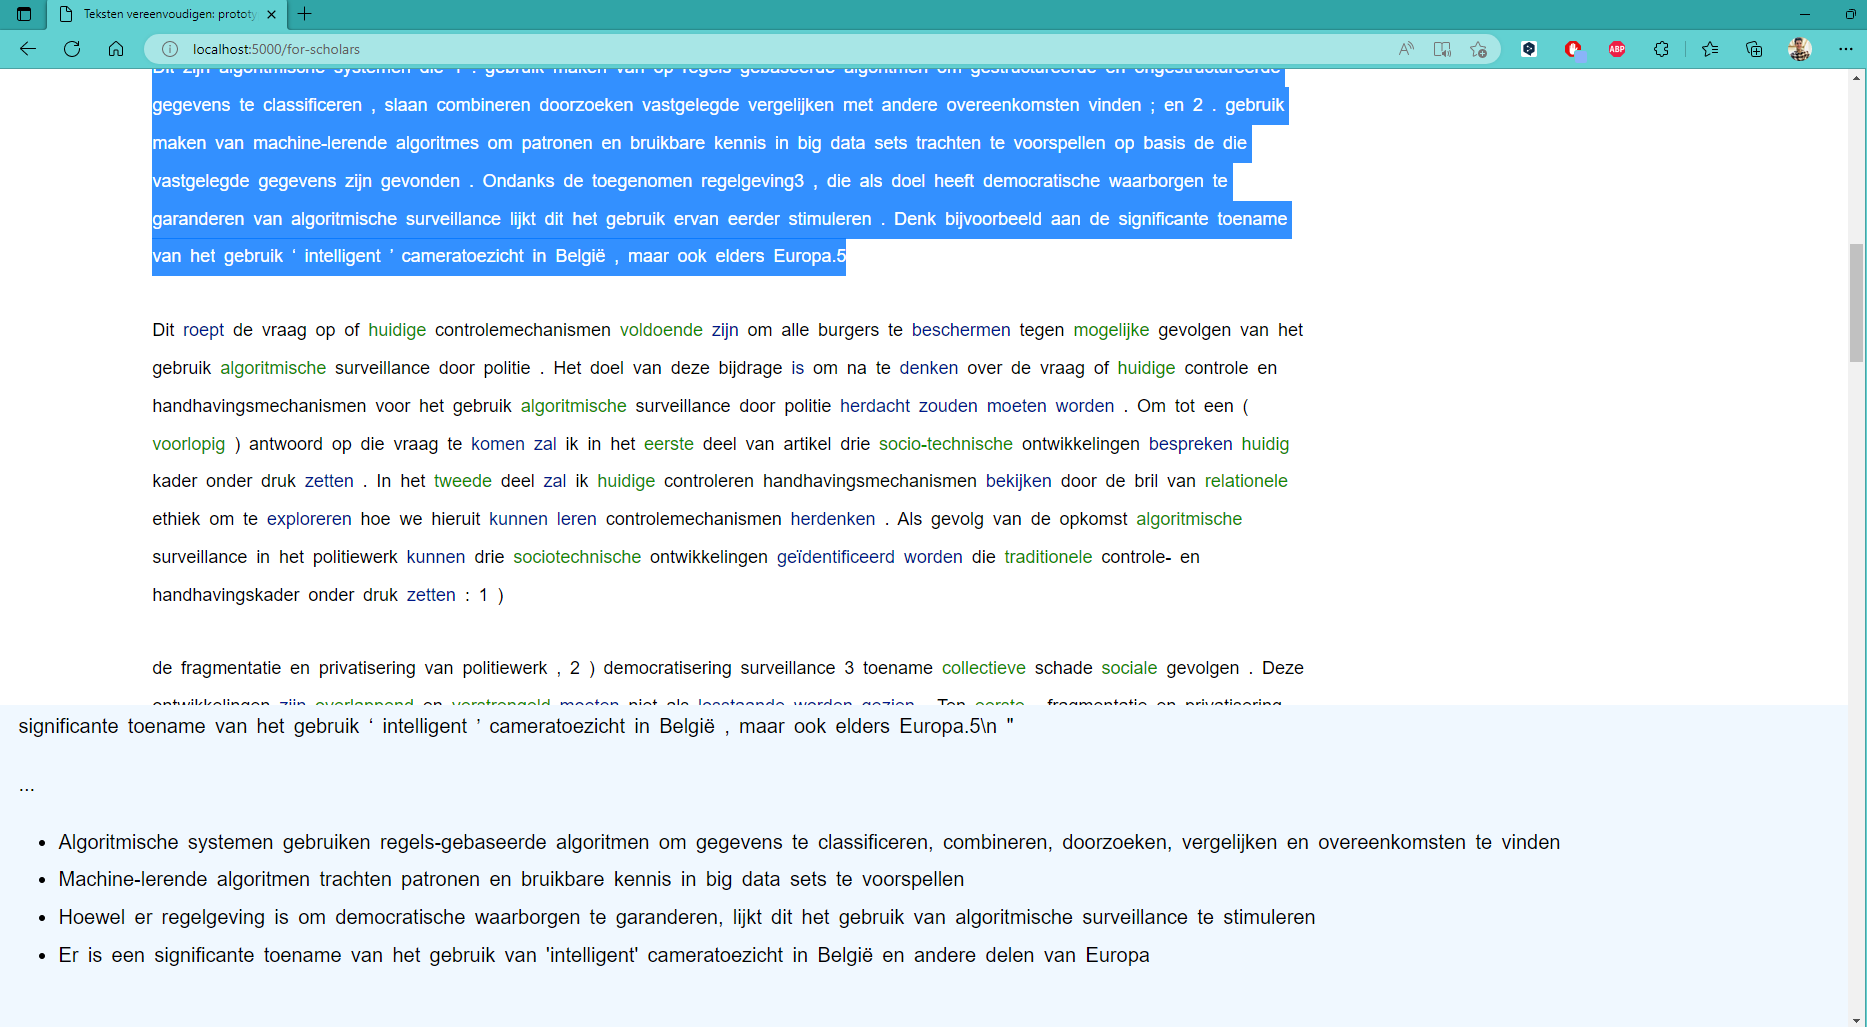
\includegraphics[width=\linewidth]{img/proto-opsomming-3.png}
		\caption{Stap 2 van een gepersonaliseerde tekstvereenvoudiging in het scholierencomponent.}
		\label{img:proto-scholieren-step-3}
	\end{figure}
\end{center}

Figuren \ref{img:step-1-proto-vraagstelling} en \ref{img:step-2-proto-vraagstelling} tonen een tweede functionaliteit. Zo kunnen scholieren specifieke vragen stellen aan het prototype door middel van een gecentreerd invoerscherm.

\begin{center}
	\begin{figure}
		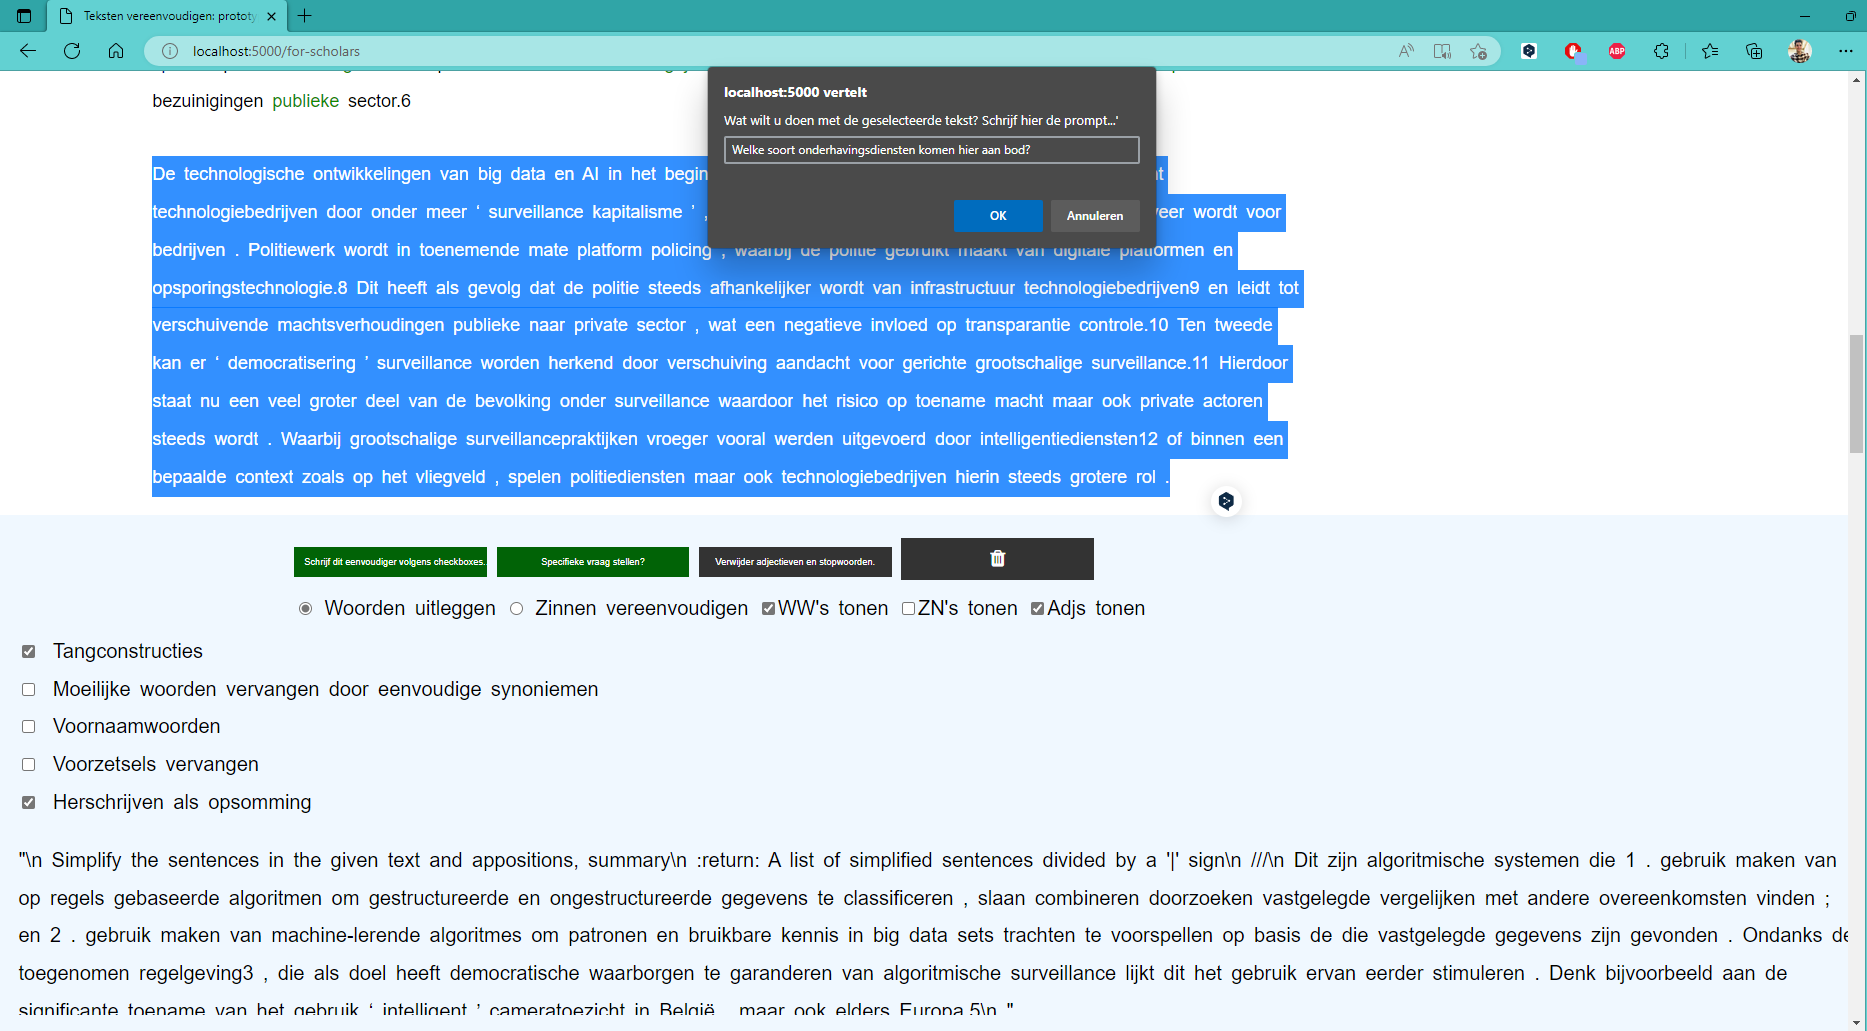
\includegraphics[width=\linewidth]{img/proto-vraagstelling-1.png}
		\caption{Stap 1 bij het stellen van een specifieke vraag bij gemarkeerde tekst.}
		\label{img:step-1-proto-vraagstelling}
	\end{figure}
\end{center}

\begin{center}
	\begin{figure}
		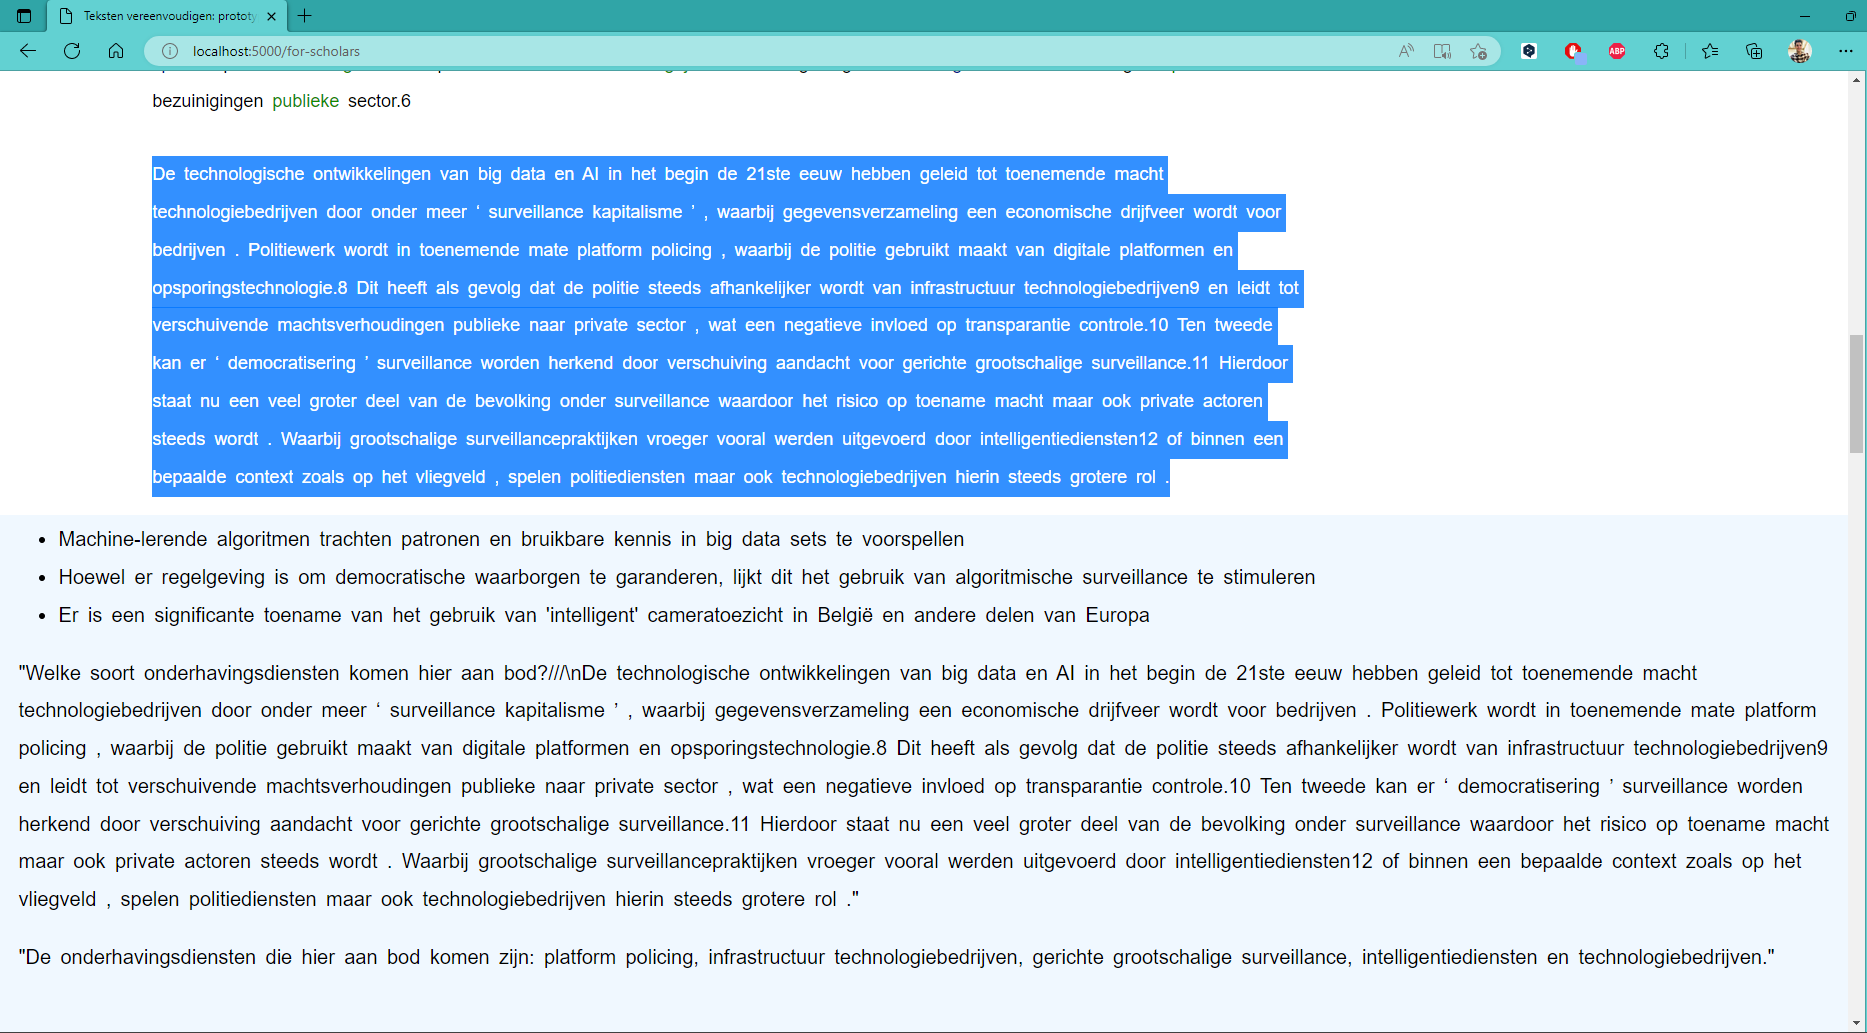
\includegraphics[width=\linewidth]{img/proto-vraagstelling-2.png}
		\caption{Stap 2 bij het stellen van een specifieke vraag bij gemarkeerde tekst.}
		\label{img:step-2-proto-vraagstelling}
	\end{figure}
\end{center}

Na evaluatie en experimenten blijkt het prototype te voldoen aan de gespecificeerde \textit{must-have} functionaliteiten, zoals vastgesteld in het moscow-schema of tabel \ref{img:moscow-table}. Het onderzoek overloopt deze functionaliteiten.

\medspace

Het prototype biedt twee manieren aan om pdf-bestanden in te lezen, namelijk via OCR en via PDFMiner. Daarnaast kan plain-text ook dienen als voer voor het prototype. Dit maakt het prototype gelijkwaardig aan de uitgeteste tools.

\medspace

Alle eindgebruikers kunnen de opmaakopties van de toepassing aanpassen aan hun persoonlijke voorkeuren bij het lezen van wetenschappelijke artikelen. Alsook de opmaak van het uitvoerbestand personaliseren. De koppenstructuur, 

Ontbrekende should-haves en wont-haves.

\medspace

Tot slot bevat het prototype geen \textit{wont-have}. Zo ontbreekt het prototype een luistercomponent waarbij scholieren de vereenvoudigde tekst kunnen beluisteren. Deze functionaliteit is wel aanwezig bij E1, E2 en E3. Daarnaast is het prototype niet beschikbaar als browserextensie. Andere uitgeteste tools beschikken hier ook niet over. Tot slot is het prototype enkel in een lokale omgeving beschikbaar. Andere uitgeteste toepassingen zijn online beschikbaar. 

% Dit wordt gerealiseerd door woordenlijsten te reproduceren na een zorgvuldige handmatige selectie van moeilijke woorden. Het prototype is lokaal op te zetten met behulp van Docker, hoewel voor het gebruik ervan een internetverbinding vereist is, net als bij andere tools in tabel \ref{table:overview-tools}.